\documentclass[journal,hidelinks]{IEEEtran}
\usepackage[utf8]{inputenc}
\usepackage[
  pdftitle={A First Order Delta-Sigma A/D Converter},
  pdfauthor={Andrei Purcarus},
  pdfsubject={ECSE-534 -- Analog Microelectronics}
]{hyperref}
\usepackage{graphicx}
\usepackage[all]{hypcap}
\usepackage{cleveref}
\usepackage{indentfirst}
\usepackage[per-mode=symbol]{siunitx}
\usepackage{amsmath}

\title{ECSE-534 \\ Analog Microelectronics \\
  A First Order $\Delta \Sigma$ A/D Converter}
\author{Andrei~Purcarus,~260631911,~\IEEEmembership{McGill~University} \\ \href{mailto:andrei.purcaruscraciun@mail.mcgill.ca}{andrei.purcaruscraciun@mail.mcgill.ca}}

\begin{document}
\sloppy

\maketitle

\begin{abstract}

A first order, single bit, $\Delta \Sigma$ A/D converter was designed, simulated, laid out, and analyzed using MATLAB and Cadence. This converter was required to achieve a peak SNDR of at least $\SI{60}{\deci\bel}$ with a bandwidth of $\SI{38.22}{\kilo\hertz}$ and a full scale input range of $\pm \SI{0.2}{\volt}$. To meet these goals, a sampling frequency of $\SI{10}{\mega\hertz}$ was used, which resulted in a peak SNDR of $\SI{63.7303}{\deci\bel}$ in a system level simulation, a peak SNDR of $\SI{65.4429}{\deci\bel}$ in a schematic level simulation, and a peak SNDR of $\SI{60.3449}{\deci\bel}$ in a layout level simulation. The A/D converter therefore satisfies all the requirements.

\end{abstract}

\section{Introduction}

\IEEEPARstart{T}{his} report follows the design, simulation, layout, and analysis of a first order, single bit, low pass $\Delta \Sigma$ A/D converter using a 0.13 micron process from IBM. We used MATLAB and Simulink to perform system level simulations, and Cadence to perform circuit level simulations and layout. The converter was required to meet the following specifications:
\begin{itemize}
  \item Bandwidth: $(1 + \alpha) \cdot \SI{20}{\kilo\hertz}$, where $\alpha =$ (last 3 digits of student ID) / 1000.
  \item SNDR (peak): \SI{60}{\deci\bel} ($>$ 10 bits).
  \item Input Voltage Range: $\SI{\pm 0.2}{\volt}$ relative to AGND.
  \item Power Dissipation: Minimum.
\end{itemize}
In addition, we were assigned a supply voltage of $\SI{1.2}{\volt}$ and an analog ground voltage of AGND $= \SI{0.6}{\volt}$.

In the previous phase of the project, we obtained a peak SNDR of $\SI{55.7223}{\deci\bel}$ for a $\SI{20}{\kilo\hertz}$ signal using a sampling frequency of $\SI{10}{\mega\hertz}$ and DAC output levels of $\SI{0.2}{\volt}$/$\SI{1.0}{\volt}$. Since this did not meet the specifications, we first performed a more detailed Simulink simulation to better model the system under test. Then, we mapped the system to a circuit, laid it out, and performed a circuit level simulation using Cadence. Finally, we analyzed the performance of the converter and verified that it meets the specifications.

\section{System Level Simulation}

We first simulated the ADC at the system level. We began by calculating the requirements of our system. From our student ID, we can determine that $\alpha = 0.911$, which means that our bandwidth is $f_{3dB} = \SI{38.22}{\kilo\hertz}$. To compute our minimal SNR, we assume that the power of the noise in our system will be about equal to the power of the signal harmonics. Thus, we require SNR $= 2$ SNDR, or SNR $= \SI{63}{\deci\bel}$ at the minimum. We can therefore compute our desired oversampling rate as
\[ OSR = 10^{(SNR_{peak} - 2.61)/30} = 103.04 \]
Using this result, we can determine that our minimum sampling frequency must be
\[ f_s = 2 \  OSR \  f_{3dB} = \SI{7.88}{\mega\hertz} \]
To allow for some margin, we chose $f_s = \SI{10}{\mega\hertz}$.

Next, we set up the simulation in Simulink, as shown in \Cref{fig:sim_diagram}. This model takes into account several non-ideal circuit parameters in order to provide more accurate results. It includes the $kT/C$ noise which is produced by the switched capacitor and the two transmission gates, with the capacitance $C$ chosen to be $\SI{1}{\pico\farad}$ as a starting point and the resistance $R$ chosen to be twice the worst case on resistance of our transmission gate, as given in \Cref{fig:transmission_gate_ron}. The model also includes the integrator and comparator input referred noise, which was modeled by fitting the data in \Cref{fig:folded_cascode_ac_noise,fig:comparator_ac_noise} to a curve of the form SND $= a + b / s$ to account for both thermal and flicker noise. It also takes into account the integrator offset, the comparator offset, and the finite DC gain of the operational amplifier.

\begin{figure}[!htb]
  \centering
  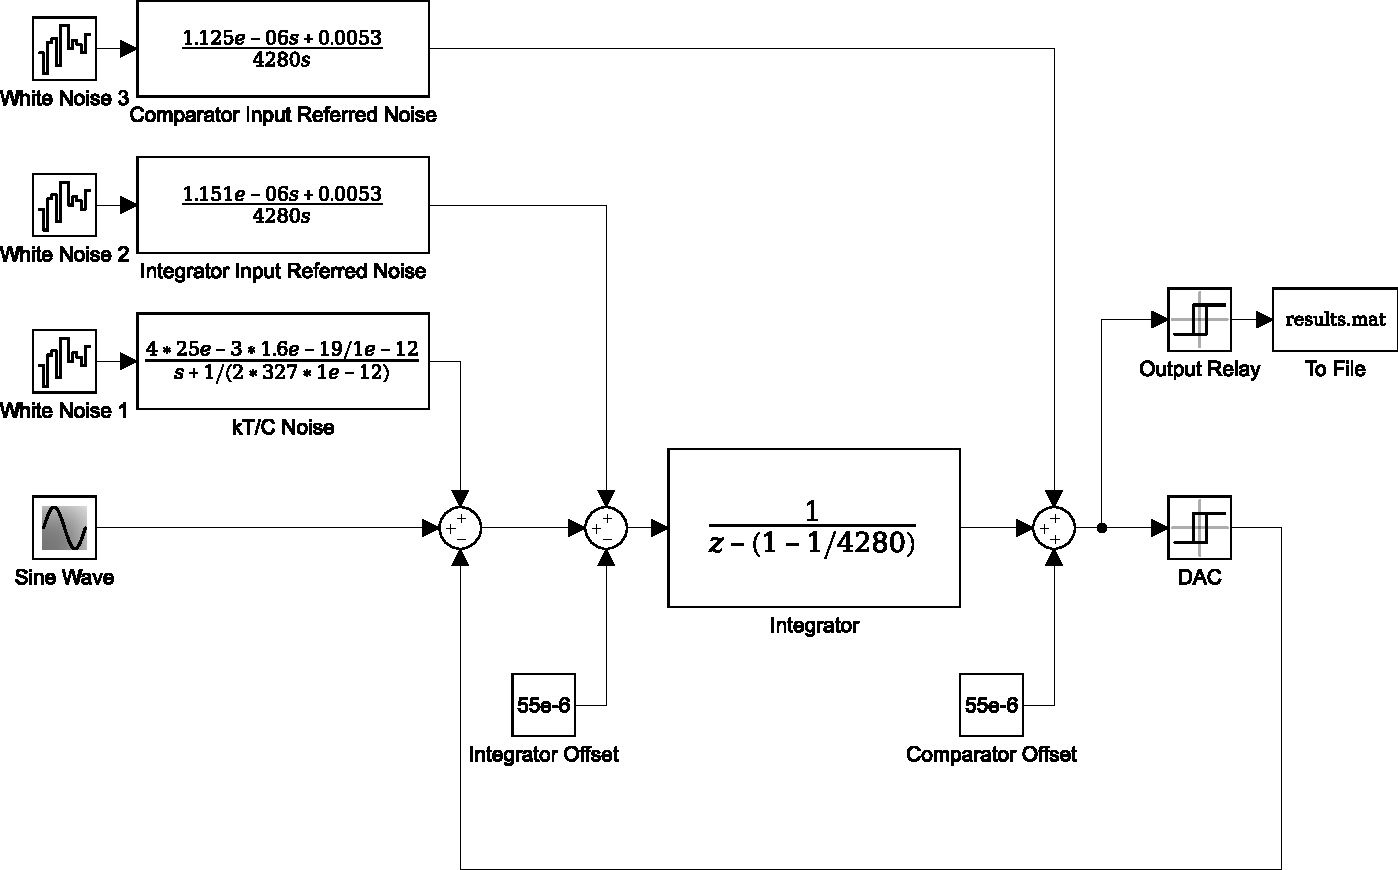
\includegraphics[width=\columnwidth]{simulation/adc.pdf}
  \caption{A system level block diagram of the $\Delta \Sigma$ A/D converter.}
  \label{fig:sim_diagram}
\end{figure}

We used a $\SI{0.2}{\volt}$ amplitude sine wave with a DC offset of $\SI{0.6}{\volt}$ as our input to the system, and we sampled this input at a rate of $\SI{10}{\mega\hertz}$. In addition, we used an input frequency of $\SI{20}{\kilo\hertz}$ to push any harmonics out of our bandwidth. For all our simulations, we used a duration of $\SI{2.1}{\milli\second}$, discarding the first $\SI{0.1}{\milli\second}$ and obtaining frequency bins of $\SI{500}{\hertz}$ each for our SNDR calculations.

To find the peak SNDR, we swept the amplitude of the DAC output around a DC offset of $\SI{0.6}{\volt}$. The results are shown in \Cref{fig:sim_sndr_vs_dac}. From this plot, we can see that the peak SNDR of $\SI{65.7803}{\deci\bel}$ occurs when the DAC output amplitude is $\SI{0.22}{\volt}$. However, it is worth analyzing the factors that contribute to this SNDR distribution. For DAC output voltages close to $\SI{0.2}{\volt}$, the minimal error at the integrator input is very close to $\SI{0}{\volt}$, and is thus susceptible to changing sign due to offset and noise. For high DAC output voltages, the maximal error at the integrator input approaches and even exceeds $\SI{0.6}{\volt}$, which can cause the operational amplifier to saturate. Thus, the best SNDR is obtained in the middle range, with the fluctuations there likely being caused by noise and the lack of samples. In order to provide a $\SI{20}{\percent}$ margin for PVT, we chose $\SI{0.24}{\volt}$, corresponding to a SNDR of $\SI{63.7303}{\deci\bel}$ and DAC outputs of $\SI{0.36}{\volt}/\SI{0.84}{\volt}$. The power spectral density of the output with these settings is shown in \Cref{fig:sim_psd}.

\begin{figure}[!htb]
  \centering
  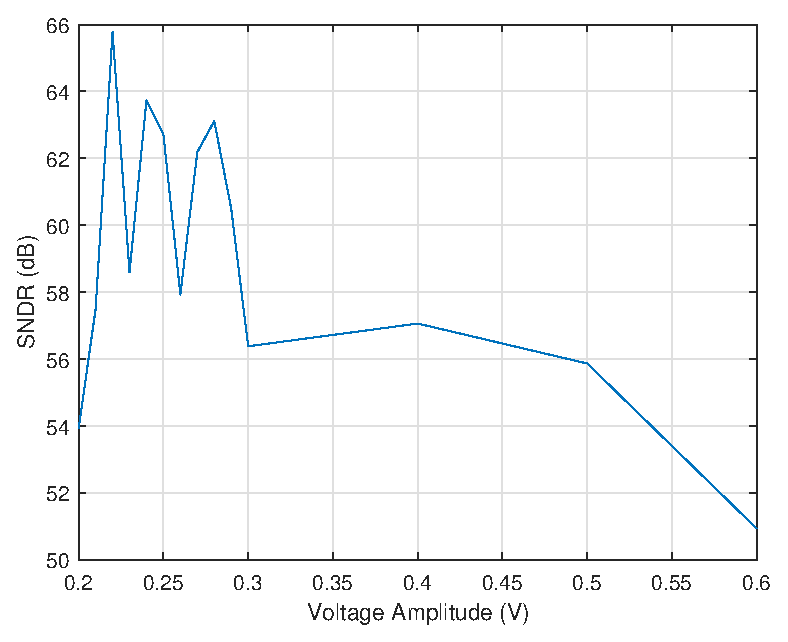
\includegraphics[width=0.8\columnwidth]{simulation/sndr_vs_dac.eps}
  \caption{SNDR vs. DAC output amplitude for the $\Delta \Sigma$ A/D converter.}
  \label{fig:sim_sndr_vs_dac}
\end{figure}

\begin{figure}[!htb]
  \centering
  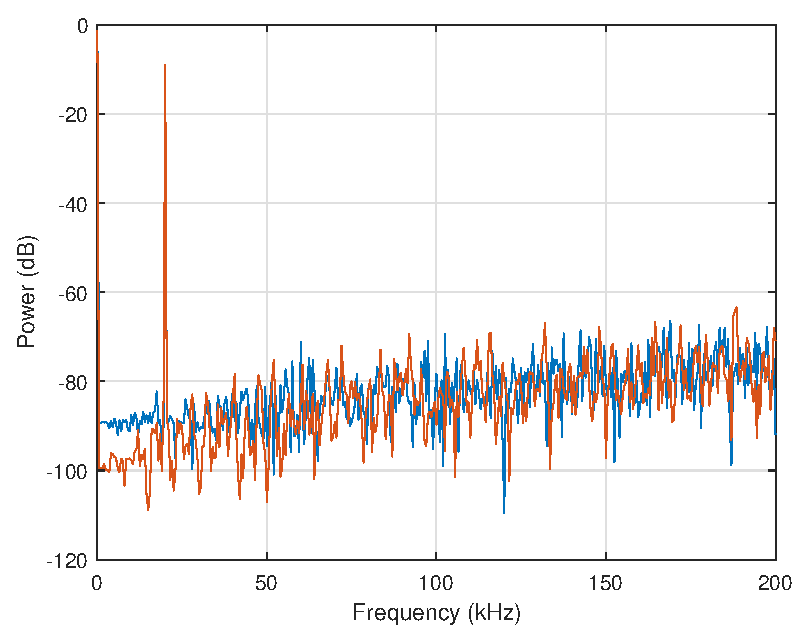
\includegraphics[width=0.8\columnwidth]{simulation/psd.eps}
  \caption{Power spectral density for the output of the $\Delta \Sigma$ A/D converter with the DAC outputs set to $\SI{0.36}{\volt}/\SI{0.84}{\volt}$.}
  \label{fig:sim_psd}
\end{figure}

\section{Circuit Level Simulation}

We next mapped the system to a circuit using Cadence. To implement the ADC, we first designed and laid out several digital components. We then implemented a transmission gate component for the switched capacitor. Next, we refitted the operational amplifier from Assignments \#2 and \#3 to implement an integrator, and we modified it to implement a comparator. Finally, we put these components together to create our ADC.

\subsection{Digital Logic}

We first implemented a basic inverter. The schematic of this implementation is shown in \Cref{fig:inverter}. Since the inverter was not required to drive large capacitances and speed was not a concern, we chose to minimize area and power consumption and used a small size of $\SI{0.4}{\micro\meter}$/$\SI{0.12}{\micro\meter}$ for our NMOS transistor. To account for the lower mobility of holes, we then chose a size of $\SI{1.0}{\micro\meter}$/$\SI{0.12}{\micro\meter}$ for our PMOS transistor. A screenshot of the layout is shown in \Cref{fig:inverter_layout}.

\begin{figure}[!htb]
  \centering
  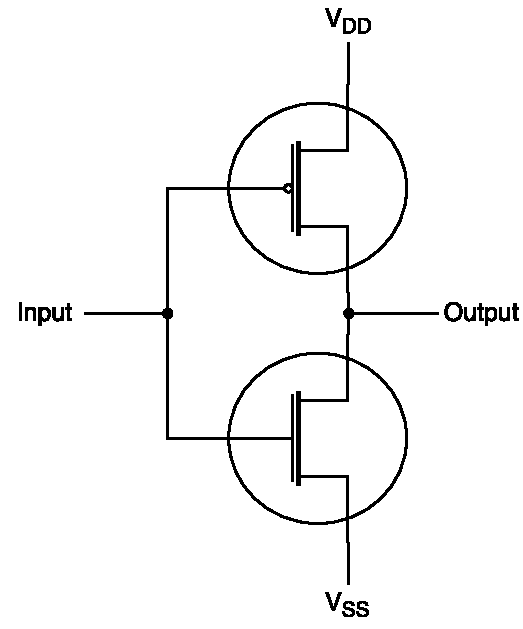
\includegraphics[height=0.5\columnwidth]{diagrams/inverter.pdf}
  \caption{A schematic of the inverter.}
  \label{fig:inverter}
\end{figure}

\begin{figure}[!htb]
  \centering
  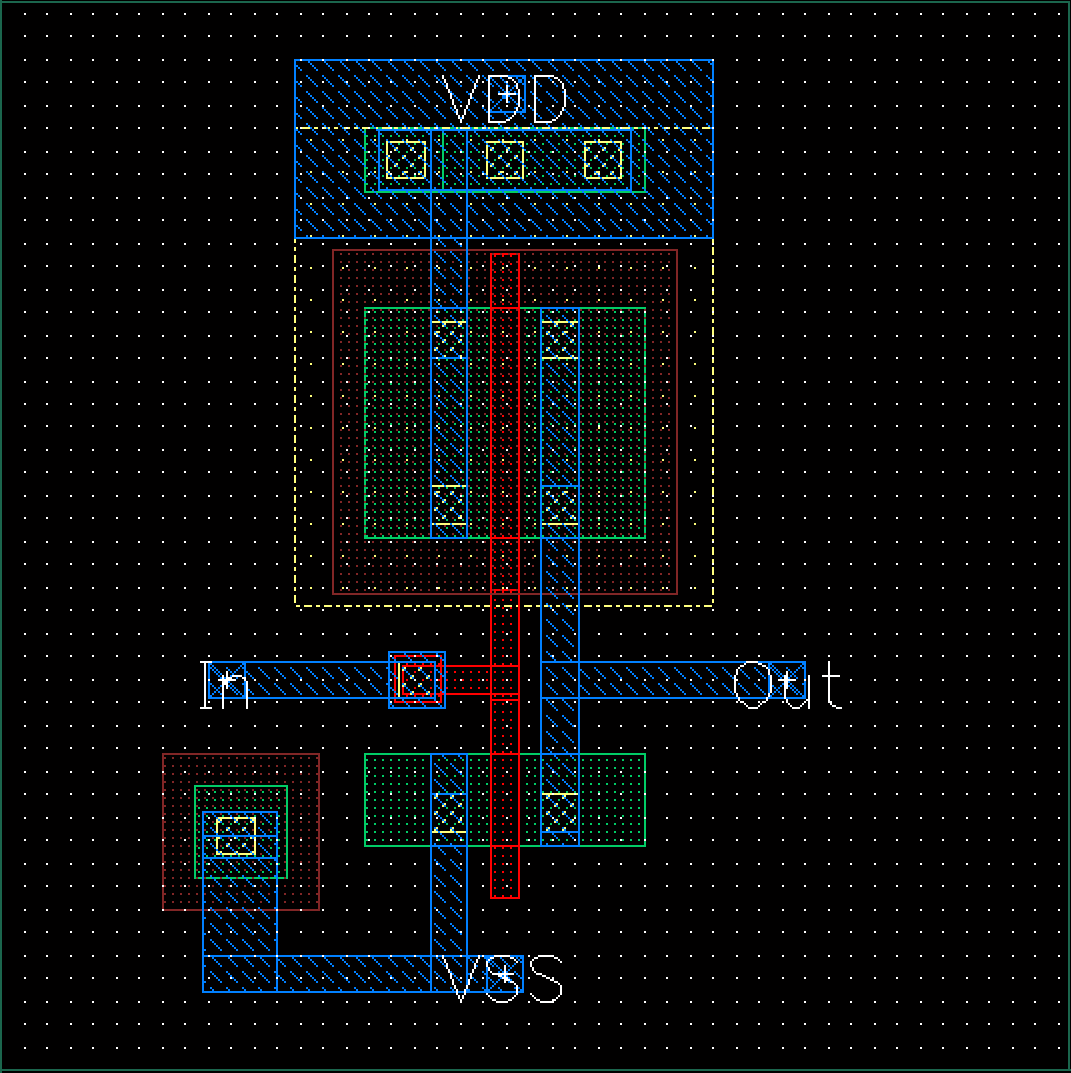
\includegraphics[width=0.8\columnwidth]{layout/inverter.png}
  \caption{A screenshot of the layout for the inverter.}
  \label{fig:inverter_layout}
\end{figure}

Then, we implemented a two-input NOR gate. The schematic of this implementation is shown in \Cref{fig:nor_gate}. To match the speed of the inverter, we selected the size of the NMOS transistors to be $\SI{0.4}{\micro\meter}$/$\SI{0.12}{\micro\meter}$. Since the PMOS transistors are in series, we used a larger size of $\SI{2.0}{\micro\meter}$/$\SI{0.12}{\micro\meter}$ to provide an equivalent size to the PMOS transistor of the inverter. A screenshot of the layout is shown in \Cref{fig:nor_gate_layout}.

\begin{figure}[!htb]
  \centering
  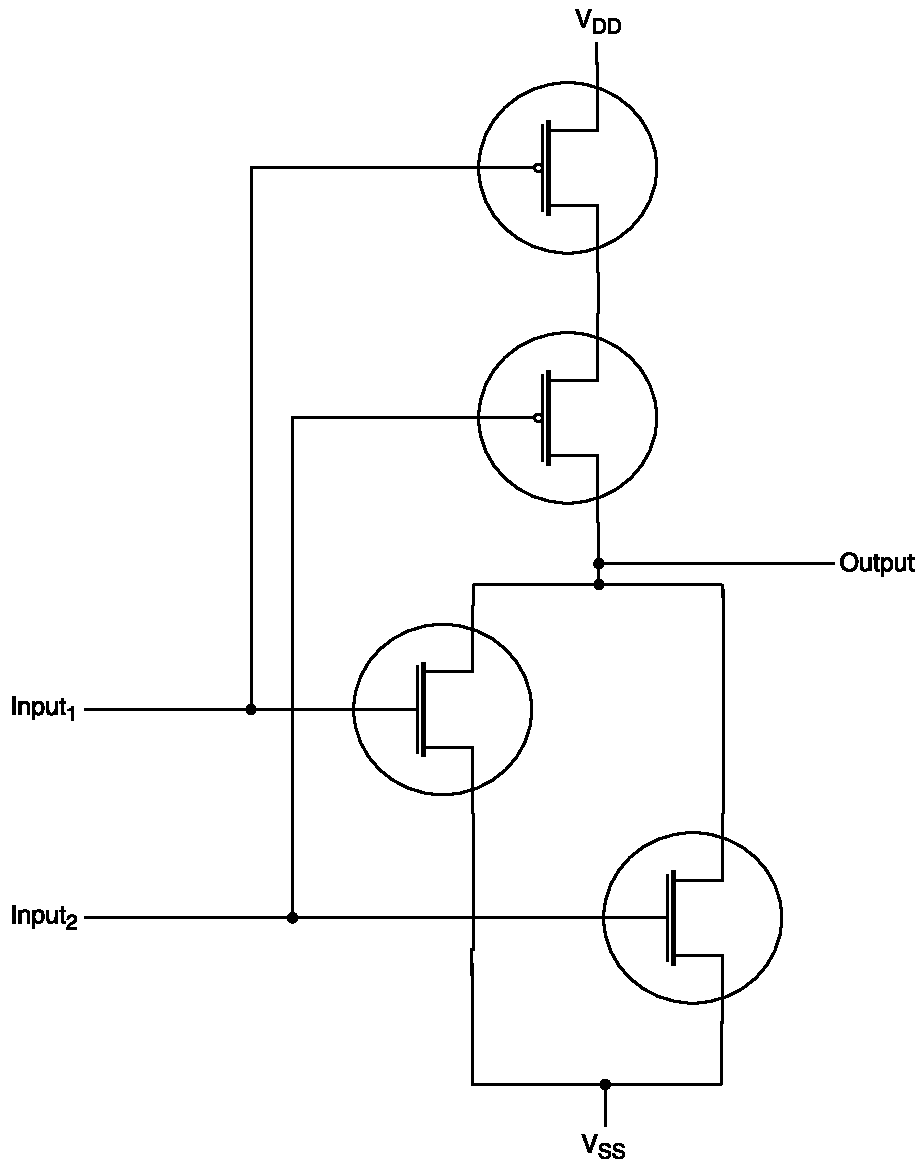
\includegraphics[height=0.7\columnwidth]{diagrams/nor_gate.pdf}
  \caption{A schematic of the two-input NOR gate.}
  \label{fig:nor_gate}
\end{figure}

\begin{figure}[!htb]
  \centering
  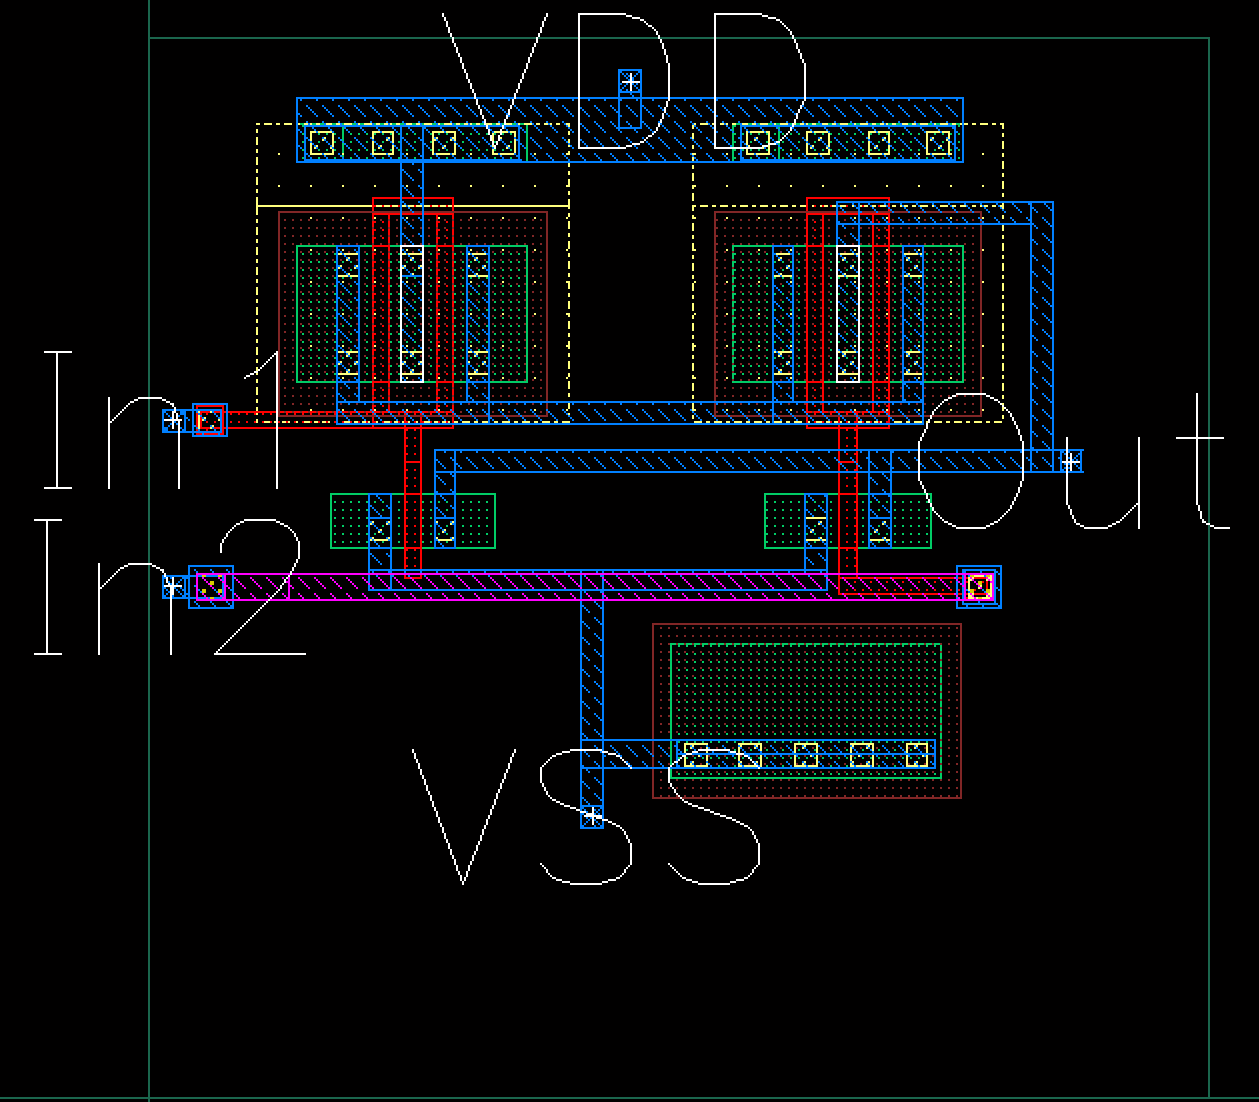
\includegraphics[width=0.8\columnwidth]{layout/nor_gate.png}
  \caption{A screenshot of the layout for the two-input NOR gate.}
  \label{fig:nor_gate_layout}
\end{figure}

Next, we implemented a three-input NOR gate. The schematic of this implementation is shown in \Cref{fig:nor_gate_3}. To match the speed of the inverter, we selected the size of the NMOS transistors to be $\SI{0.4}{\micro\meter}$/$\SI{0.12}{\micro\meter}$. Since the PMOS transistors are in series, we used a larger size of $\SI{3.0}{\micro\meter}$/$\SI{0.12}{\micro\meter}$ to provide an equivalent size to the PMOS transistor of the inverter. A screenshot of the layout is shown in \Cref{fig:nor_gate_3_layout}.

\begin{figure}[!htb]
  \centering
  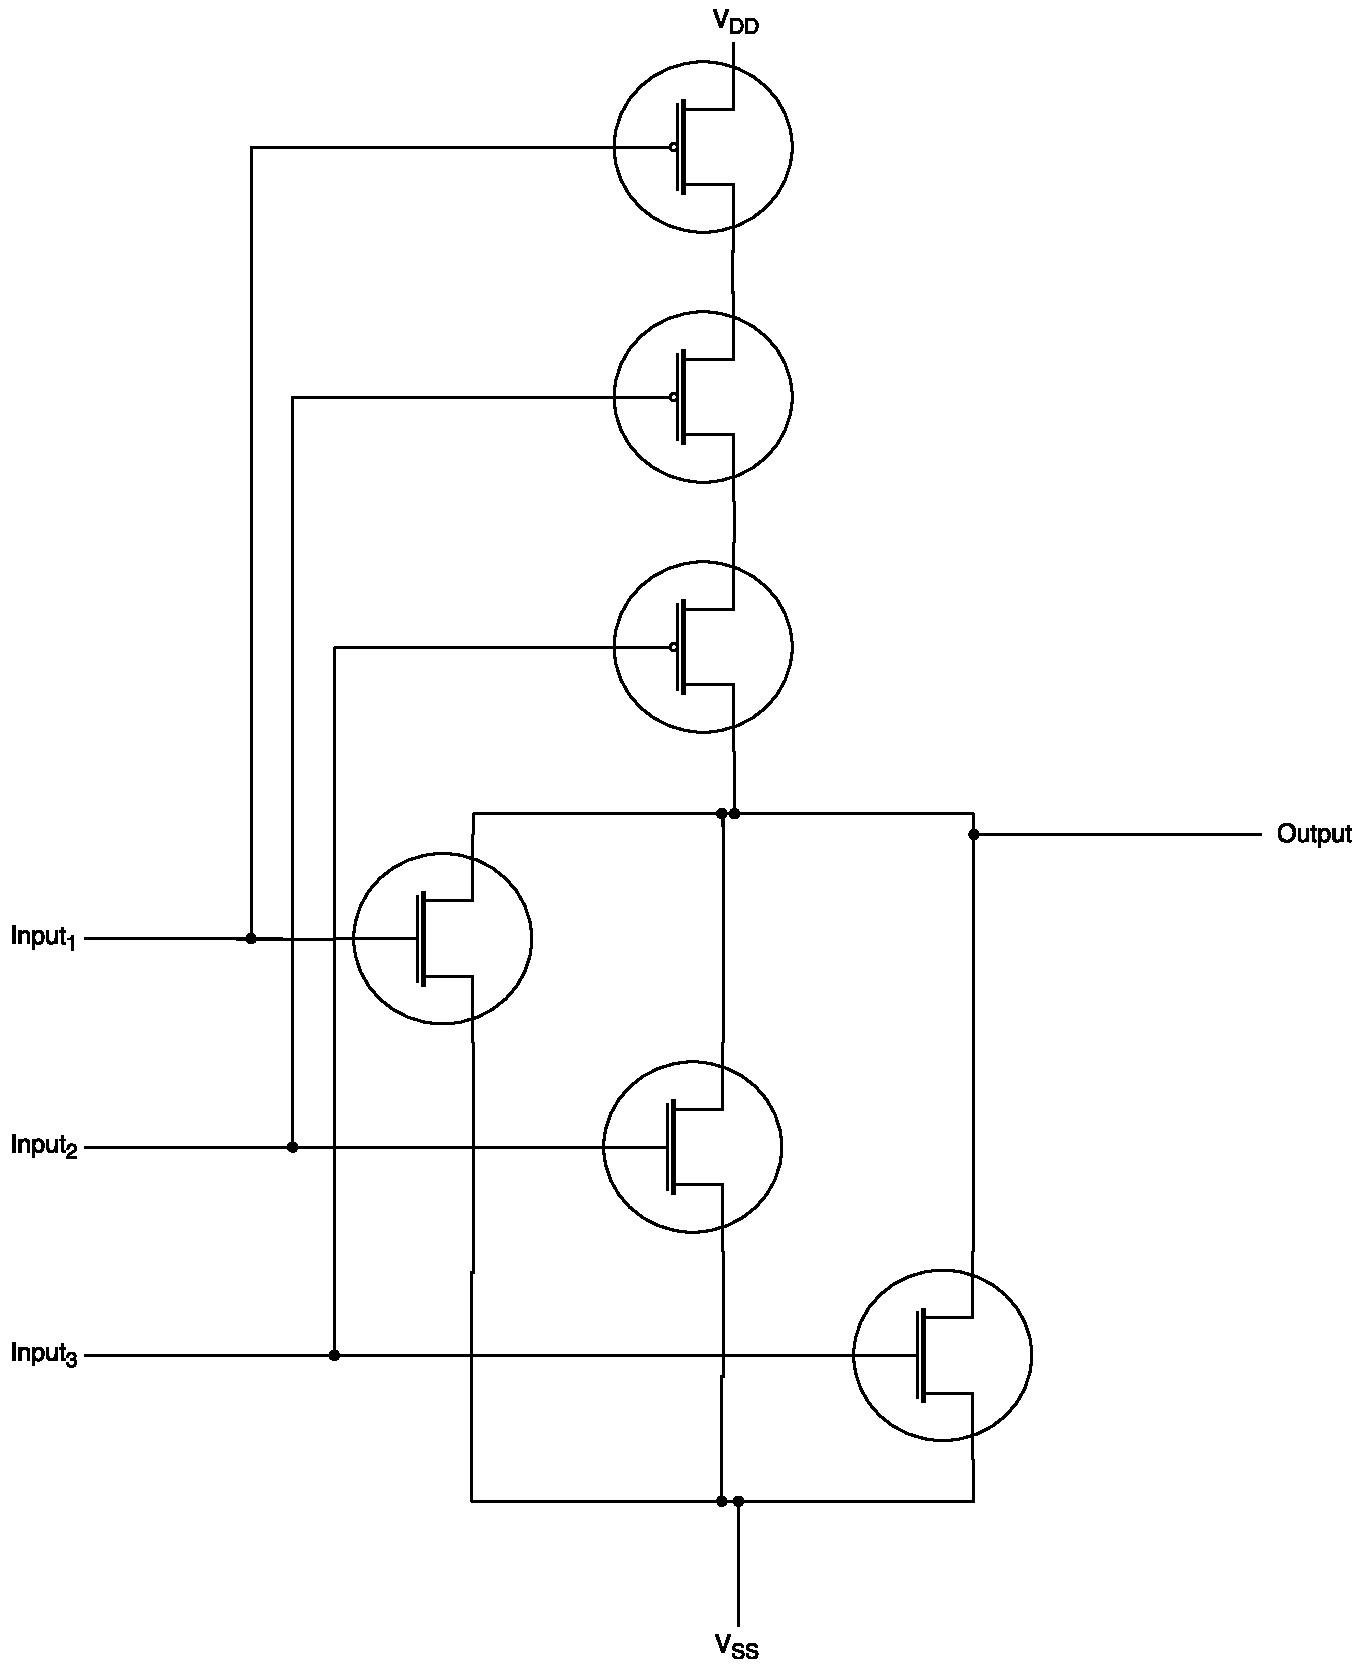
\includegraphics[height=0.8\columnwidth]{diagrams/nor_gate_3.pdf}
  \caption{A schematic of the three-input NOR gate.}
  \label{fig:nor_gate_3}
\end{figure}

\begin{figure}[!htb]
  \centering
  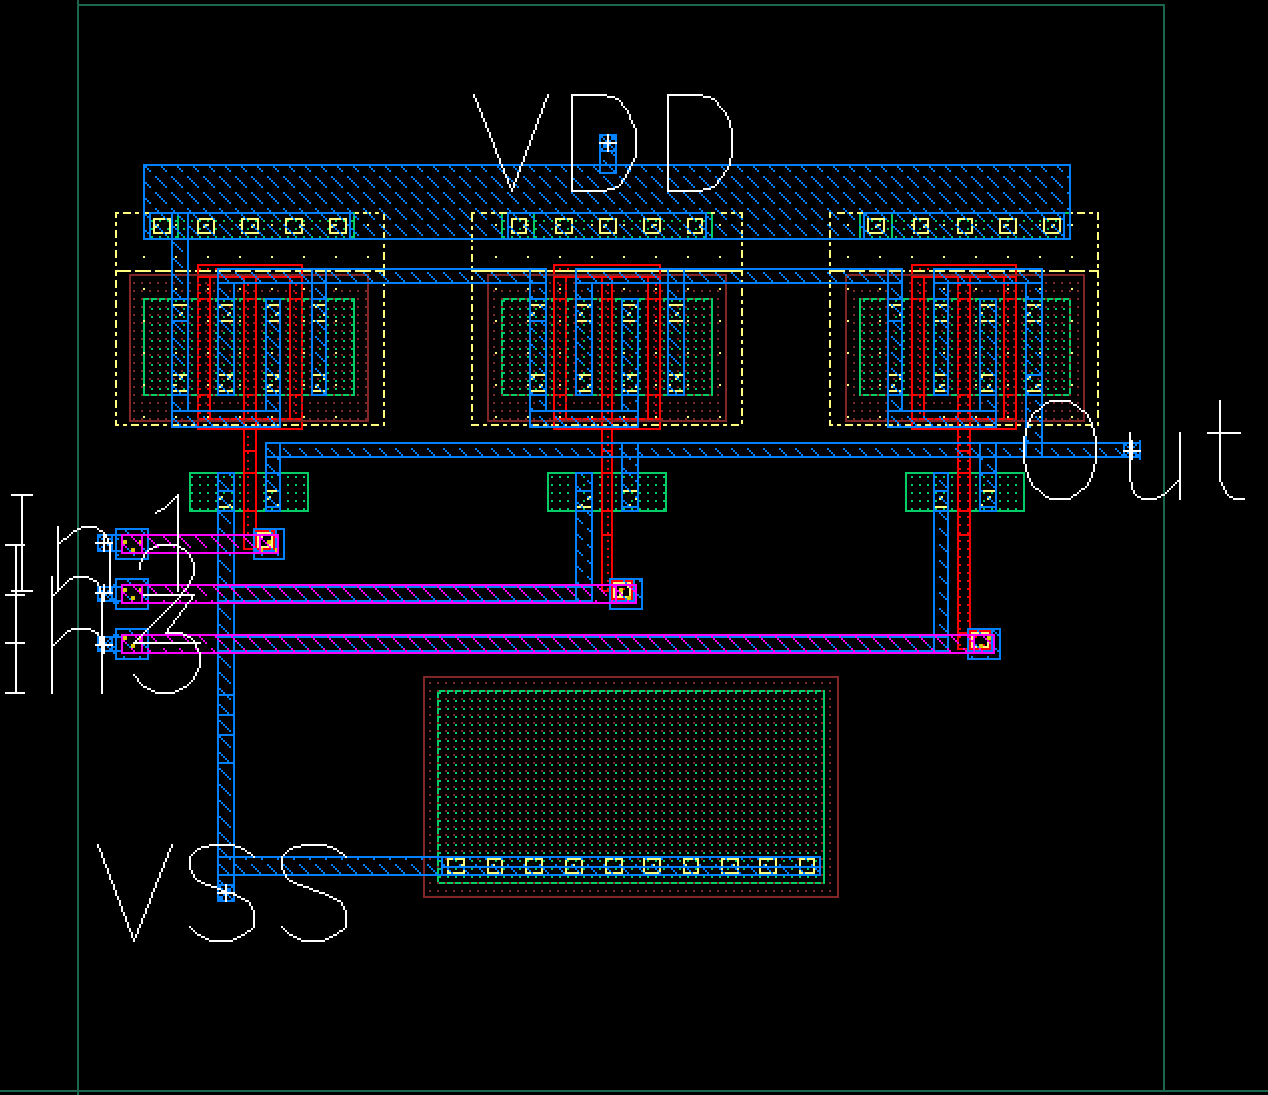
\includegraphics[width=0.8\columnwidth]{layout/nor_gate_3.png}
  \caption{A screenshot of the layout for the three-input NOR gate.}
  \label{fig:nor_gate_3_layout}
\end{figure}

Then, we implemented an edge triggered D flip-flop to serve as a register for our ADC output. The schematic of this implementation is shown in \Cref{fig:flip_flop}. A screenshot of the layout is shown in \Cref{fig:flip_flop_layout}. This circuit is triggered by the falling edge of the clock.

\begin{figure}[!htb]
  \centering
  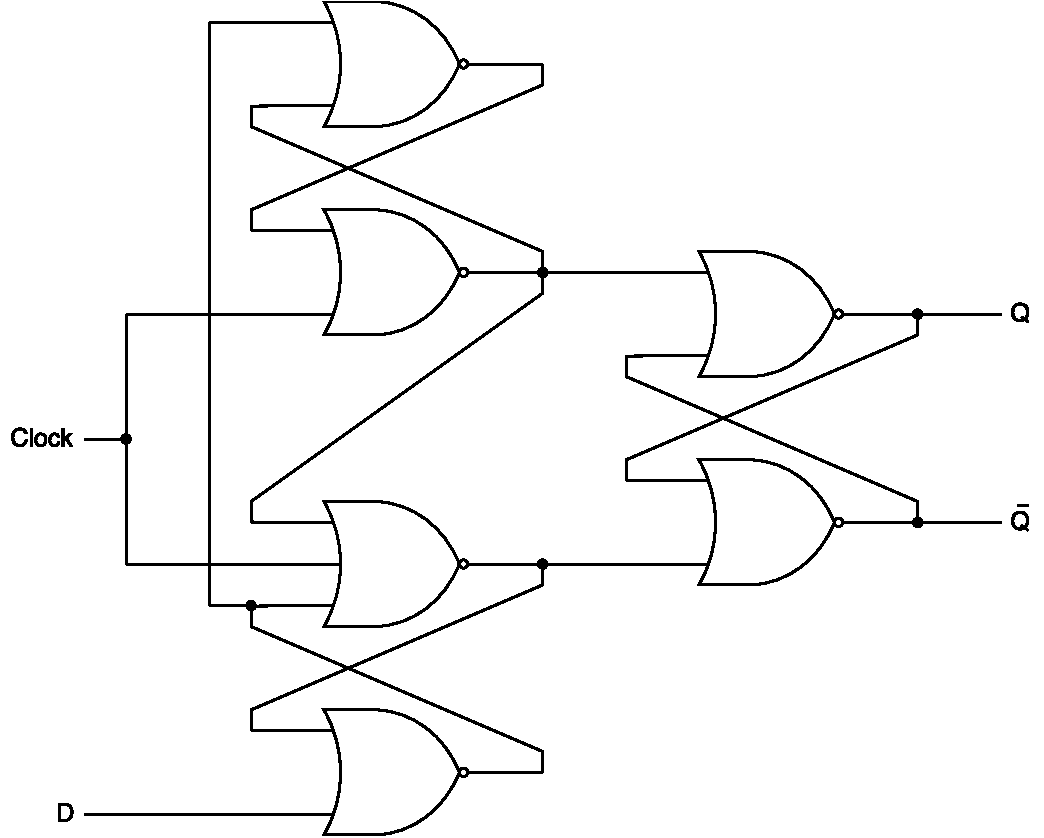
\includegraphics[width=0.8\columnwidth]{diagrams/flip_flop.pdf}
  \caption{A schematic of the D flip-flop.}
  \label{fig:flip_flop}
\end{figure}

\begin{figure}[!htb]
  \centering
  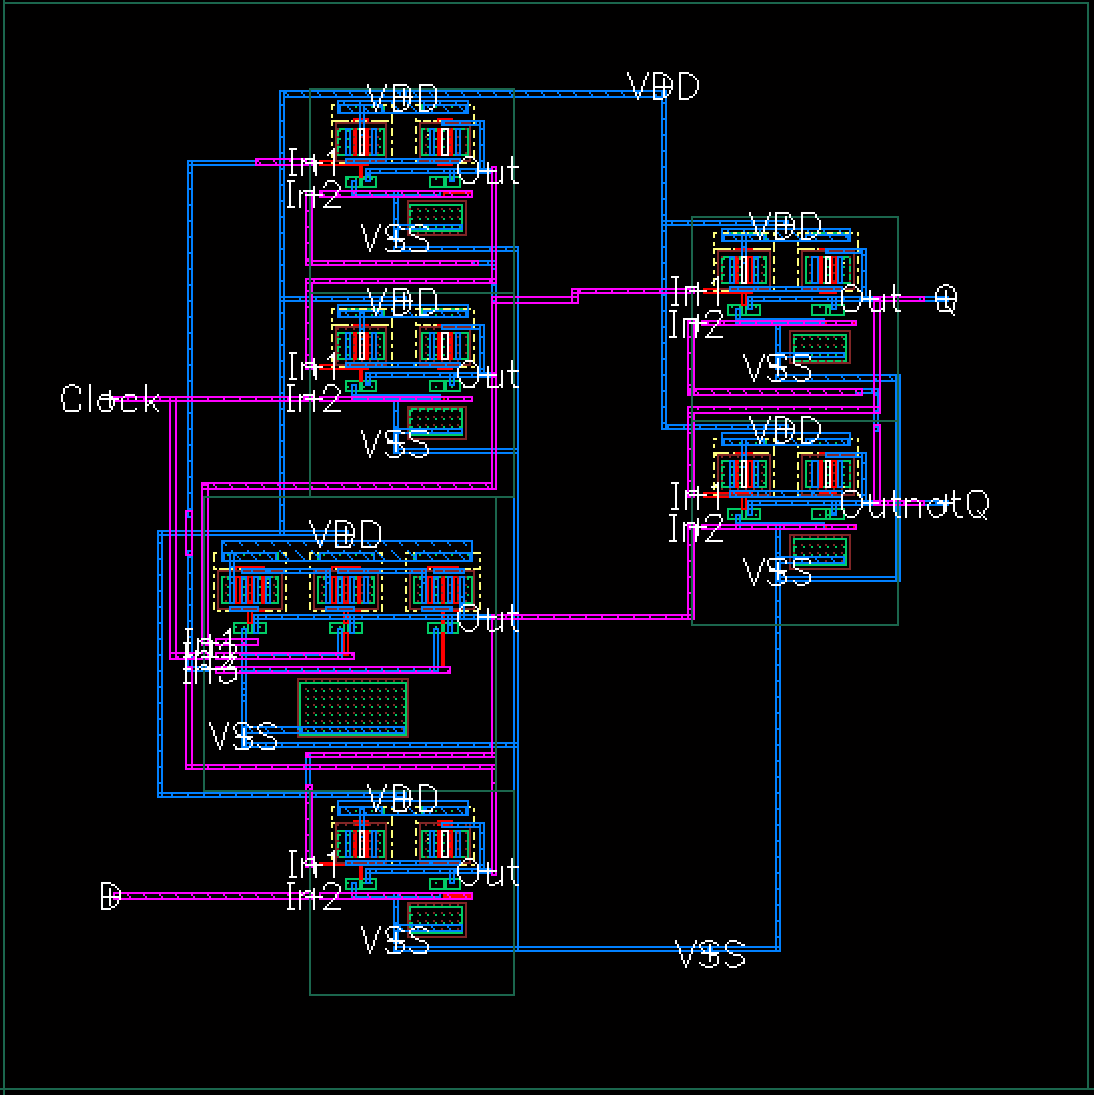
\includegraphics[width=0.8\columnwidth]{layout/flip_flop.png}
  \caption{A screenshot of the layout for the D flip-flop.}
  \label{fig:flip_flop_layout}
\end{figure}

Finally, we implemented a phase splitter in order to generate non-overlapping 2 phase clock signals that we could use to operate our switched capacitor circuit. We achieved this by negating the clock to provide the second phase and then using an SR latch and a series of buffers to ensure that the two phases never overlap. A schematic of this implementation is shown in \Cref{fig:phase_splitter}. A screenshot of the layout is shown in \Cref{fig:phase_splitter_layout}.

\begin{figure}[!htb]
  \centering
  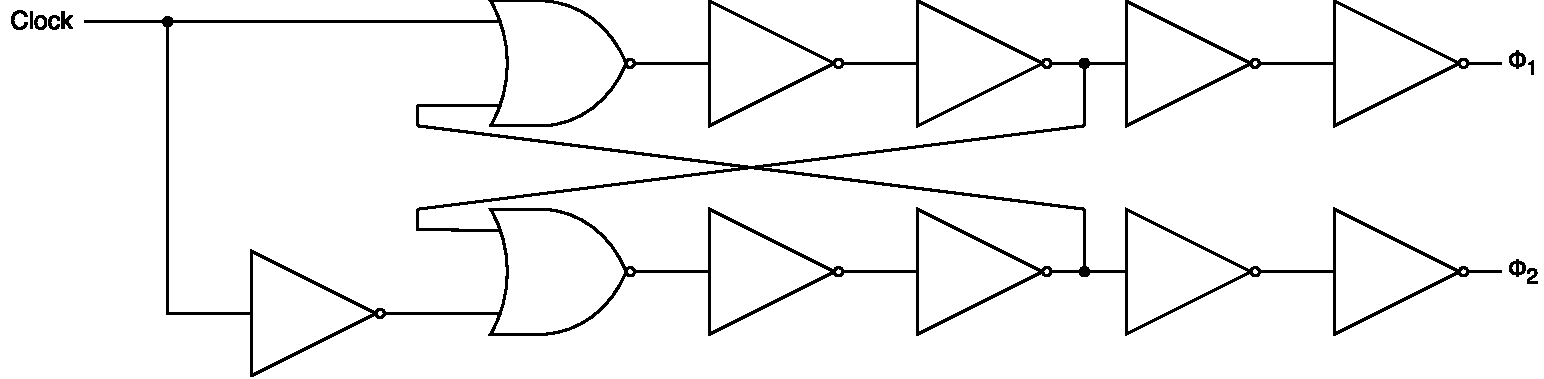
\includegraphics[width=\columnwidth]{diagrams/phase_splitter.pdf}
  \caption{A schematic of the phase splitter used to generate non-overlapping 2 phase clock signals.}
  \label{fig:phase_splitter}
\end{figure}

\begin{figure}[!htb]
  \centering
  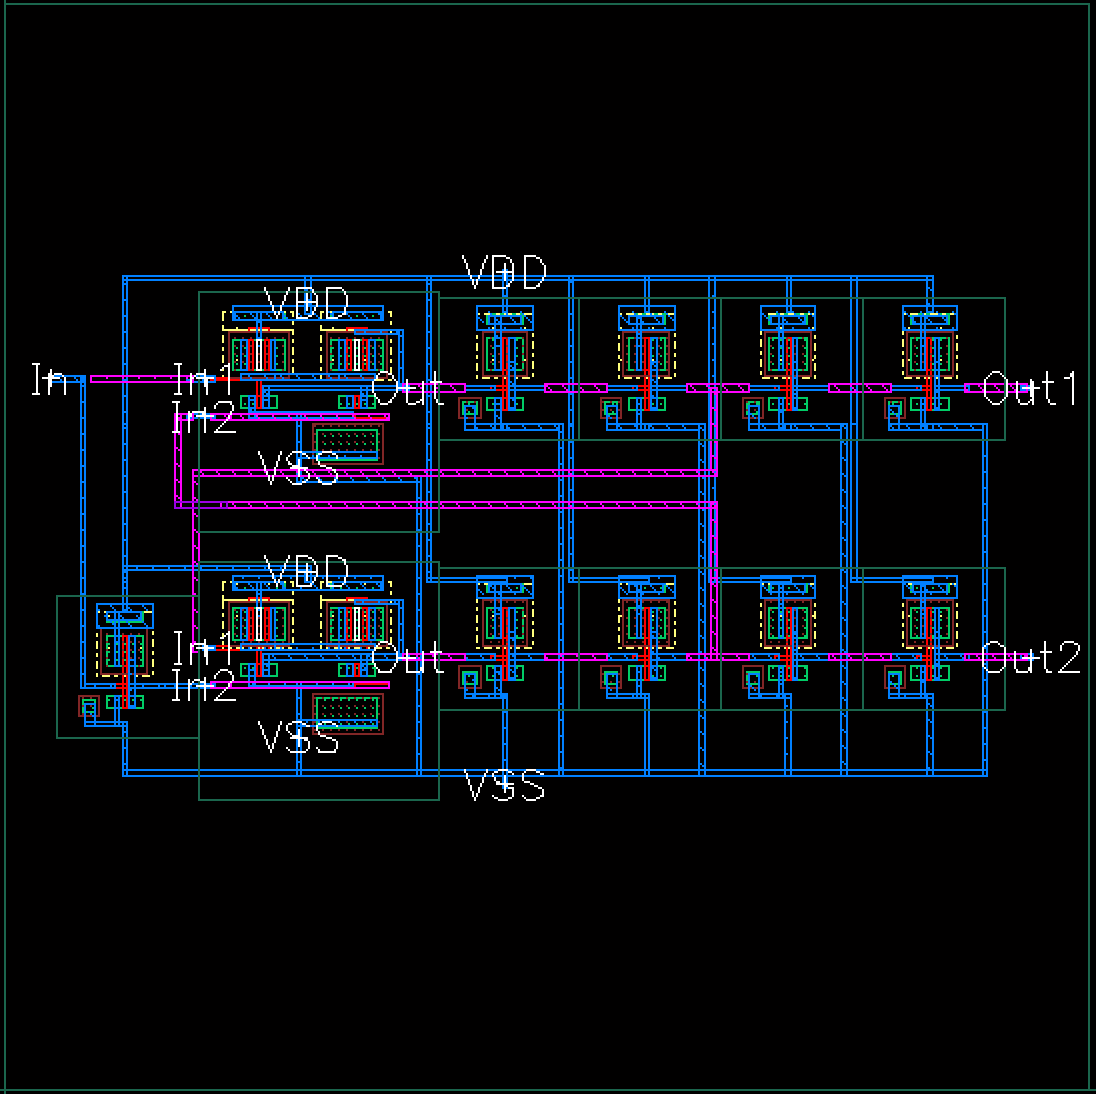
\includegraphics[width=0.8\columnwidth]{layout/phase_splitter.png}
  \caption{A screenshot of the layout for the phase splitter.}
  \label{fig:phase_splitter_layout}
\end{figure}

\subsection{Transmission Gates}

Then, we used the inverter component to implement a basic transmission gate, as shown in \Cref{fig:transmission_gate}. Since these gates would be required to drive larger capacitances, we used larger sizes of $\SI{10}{\micro\meter}$/$\SI{0.12}{\micro\meter}$ for the NMOS transistor and $\SI{25}{\micro\meter}$/$\SI{0.12}{\micro\meter}$ for the PMOS transistor. A screenshot of the layout is shown in \Cref{fig:transmission_gate_layout}.

\begin{figure}[!htb]
  \centering
  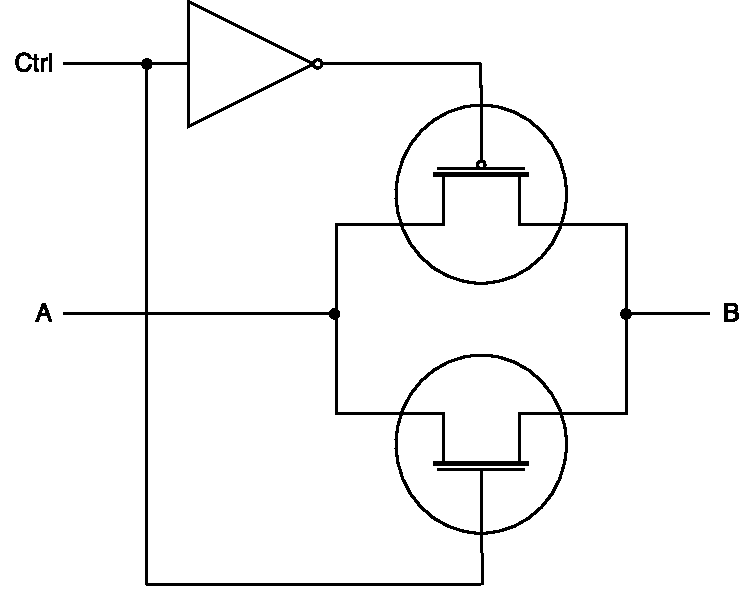
\includegraphics[height=0.5\columnwidth]{diagrams/transmission_gate.pdf}
  \caption{A schematic of the transmission gate.}
  \label{fig:transmission_gate}
\end{figure}

\begin{figure}[!htb]
  \centering
  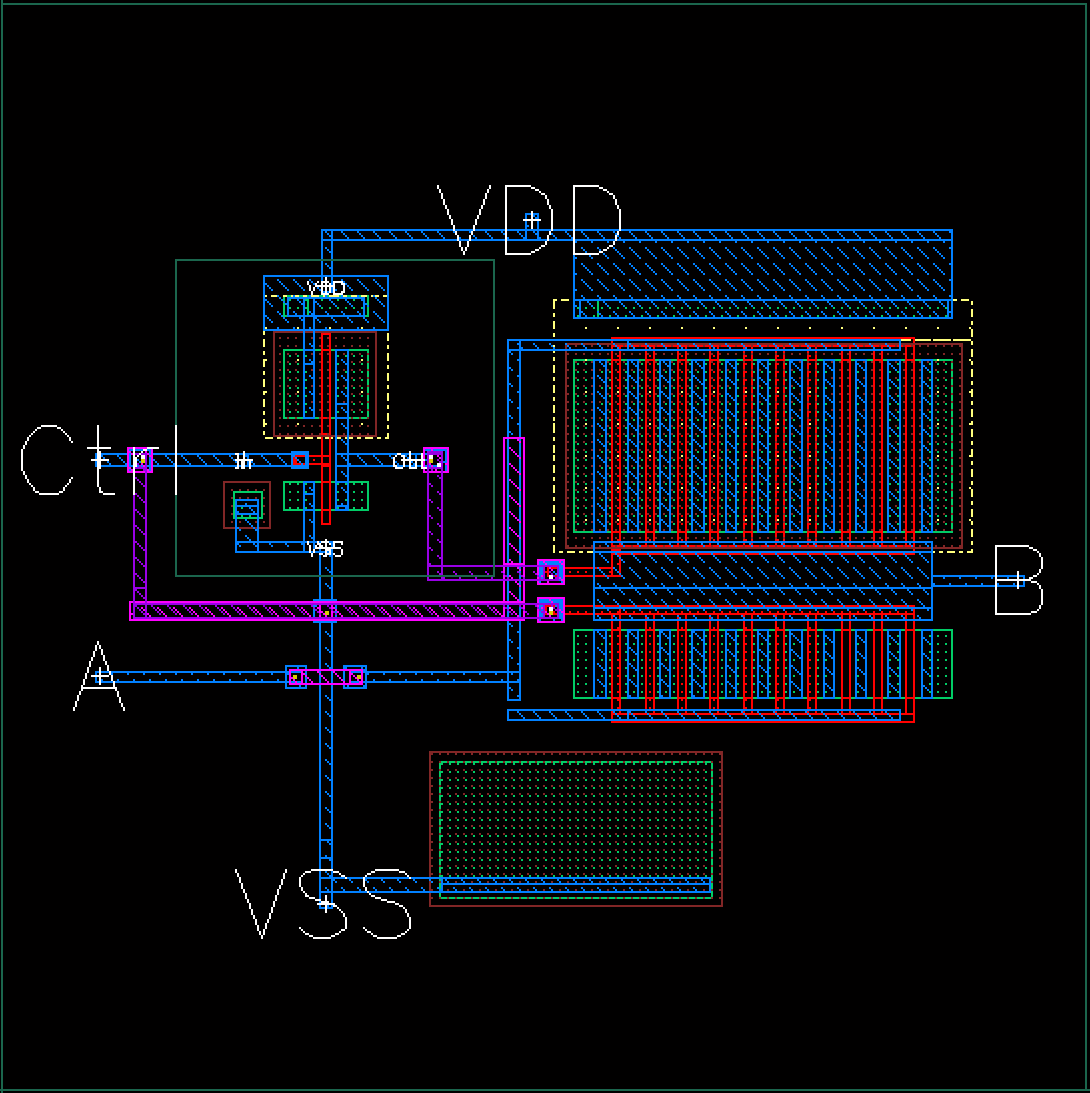
\includegraphics[width=0.8\columnwidth]{layout/transmission_gate.png}
  \caption{A screenshot of the layout for the transmission gate.}
  \label{fig:transmission_gate_layout}
\end{figure}

In order to produce a better Simulink simulation and model the $kT/C$ noise, we measured the on resistance of the transmission gate by using it to drive a $\SI{10}{\kilo\ohm}$ load and measuring the voltage drop across the gate and the current drawn by the gate for different inputs while the gate was active. The results are shown in \Cref{fig:transmission_gate_ron}, which shows that we have a maximum on resistance of $R_{on, max} = \SI{327}{\ohm}$.

\begin{figure}[!htb]
  \centering
  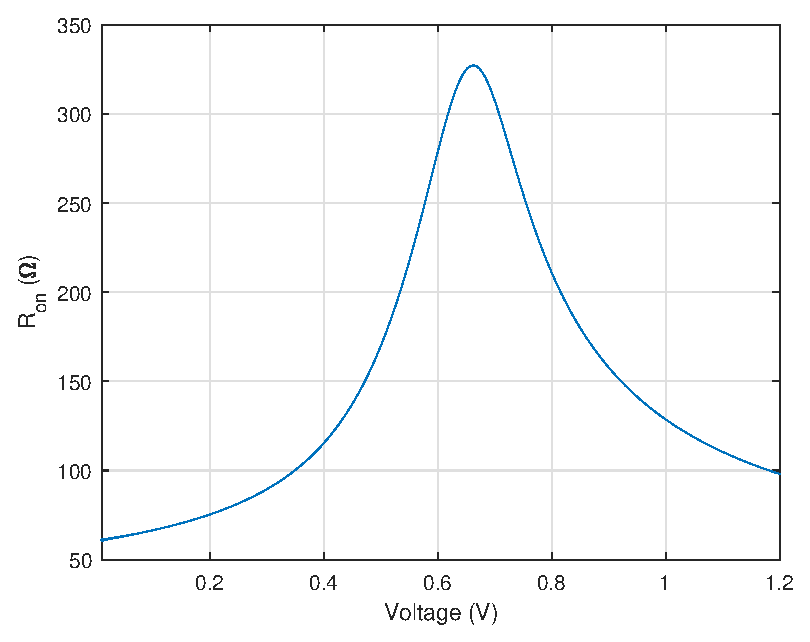
\includegraphics[width=0.8\columnwidth]{circuit/transmission_gate/ron.eps}
  \caption{$R_{on}$ vs. input voltage for an active transmission gate.}
  \label{fig:transmission_gate_ron}
\end{figure}

\subsection{Operational Amplifier}

\begin{figure*}[!htb]
  \centering
  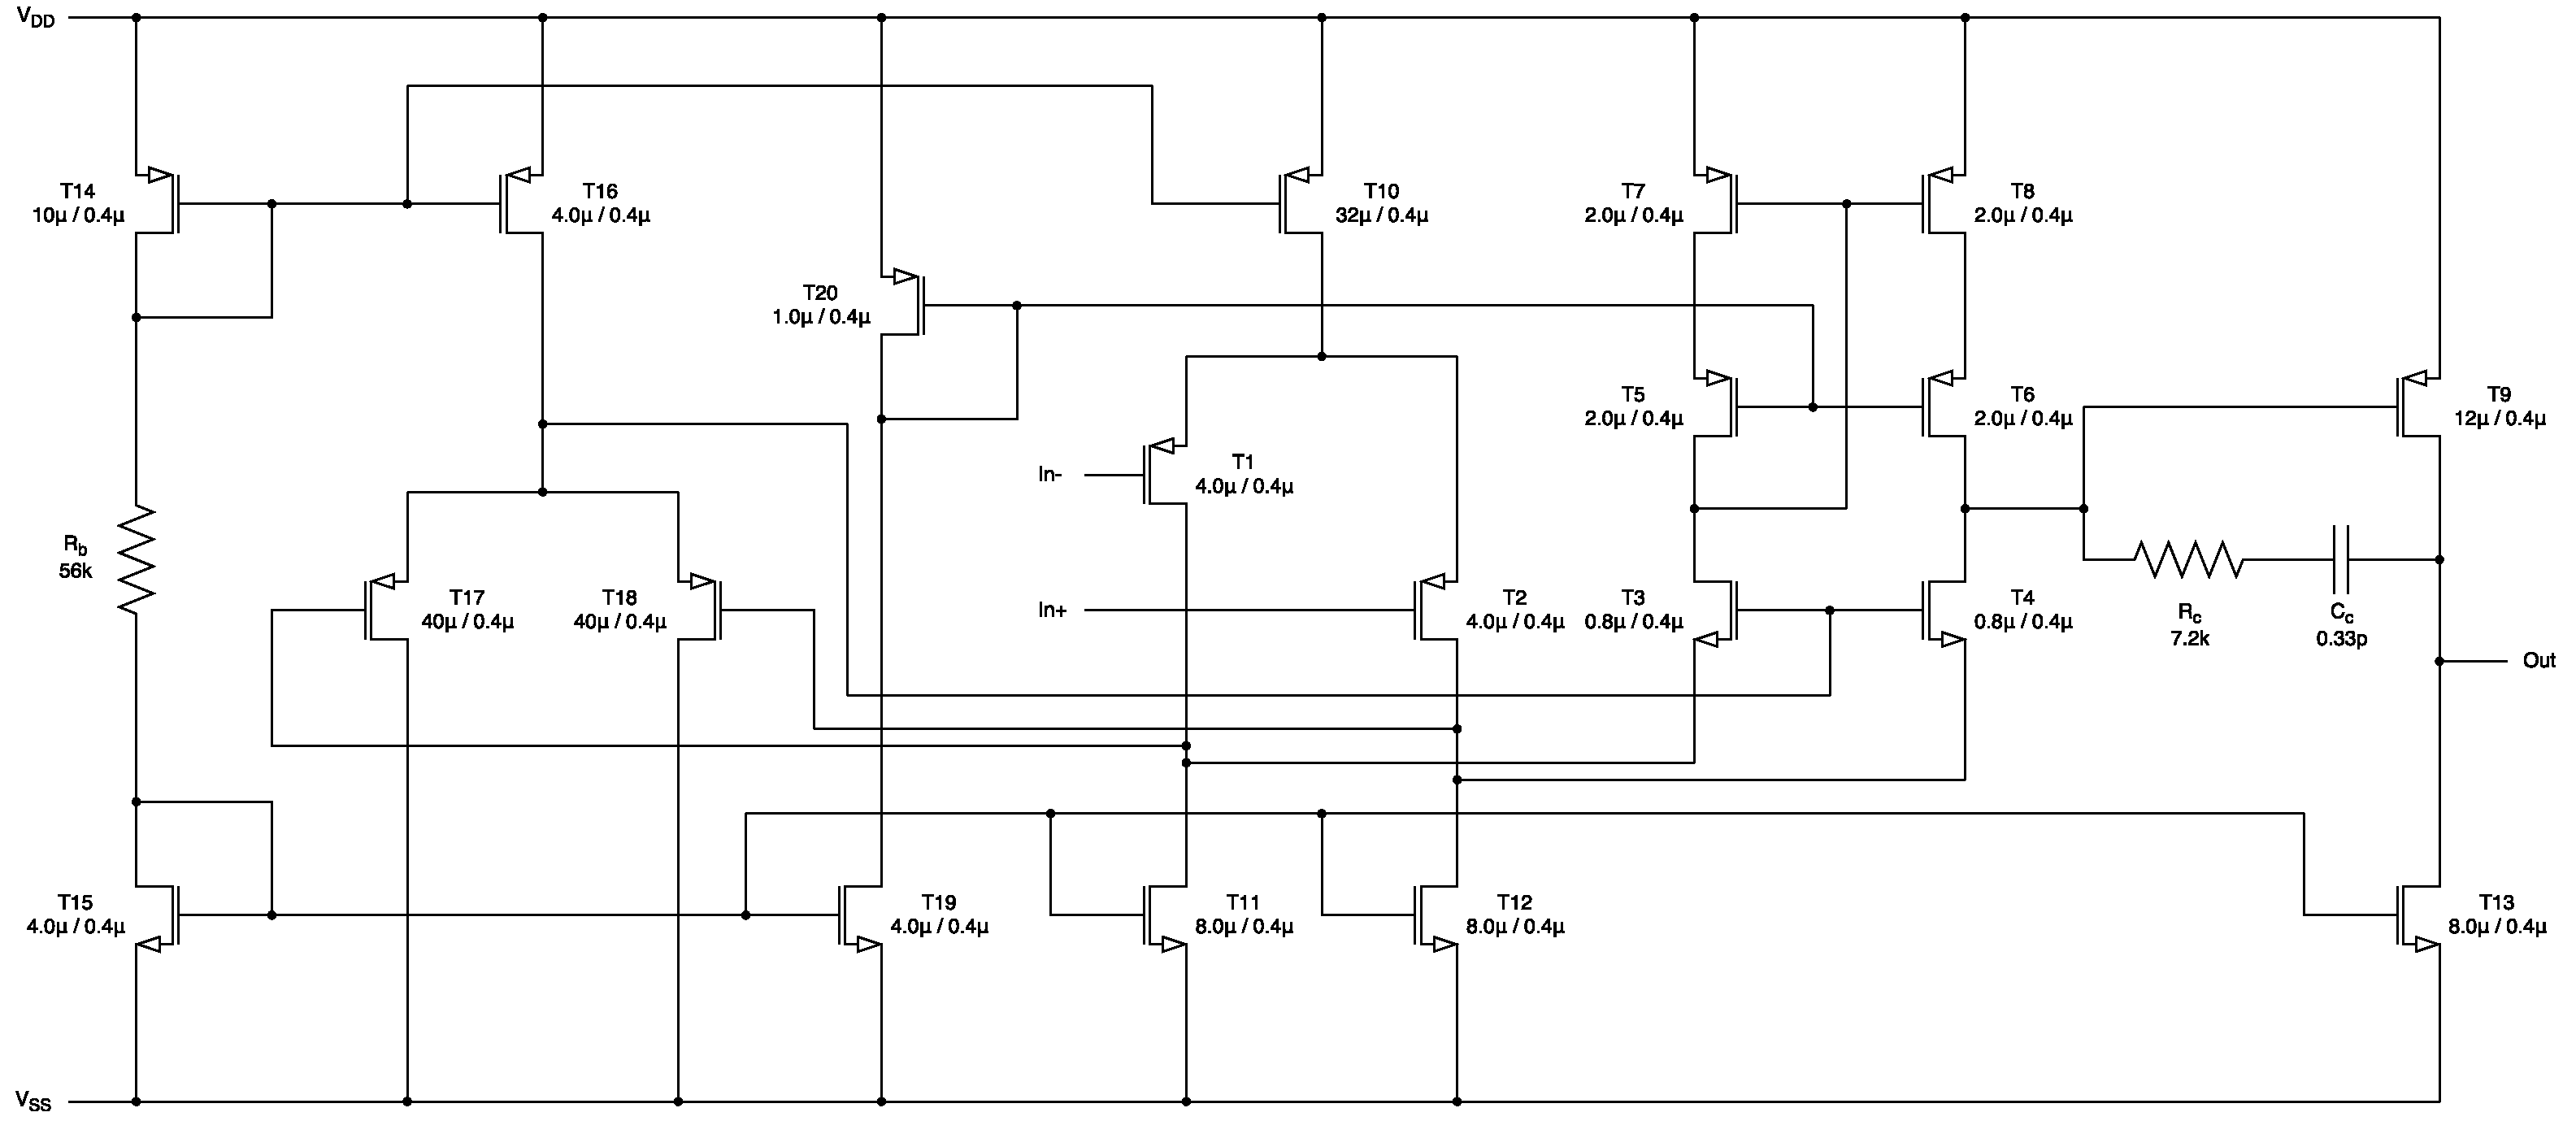
\includegraphics[width=\textwidth]{diagrams/folded_cascode.pdf}
  \caption{A schematic of the folded cascode operational amplifier.}
  \label{fig:folded_cascode}
\end{figure*}

Next, we used the operational amplifier designed in the previous assignments as an integrator. A full schematic is shown in \Cref{fig:folded_cascode}. The layout is shown in \Cref{fig:folded_cascode_layout}.

\begin{figure}[!htb]
  \centering
  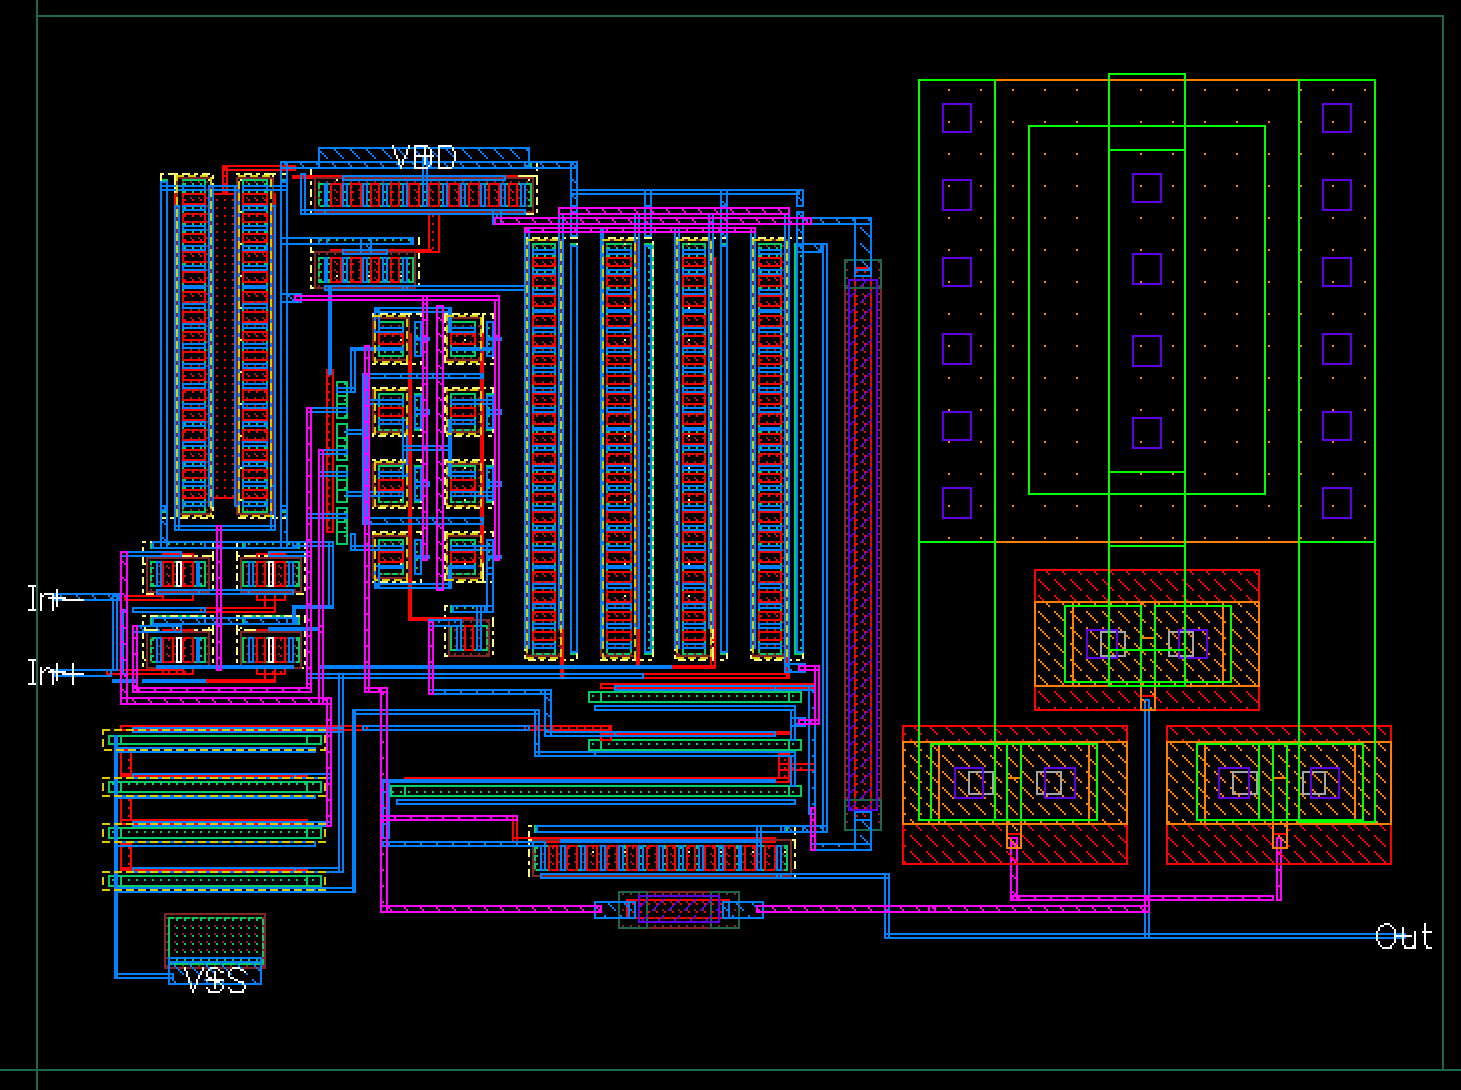
\includegraphics[width=\columnwidth]{layout/folded_cascode.png}
  \caption{A screenshot of the layout for the folded cascode operational amplifier.}
  \label{fig:folded_cascode_layout}
\end{figure}

In the interest of creating a better Simulink model, we measured several parameters of the amplifier. We found an offset voltage of $V_{os} = \SI{55}{\micro\volt}$, a DC gain of $A = \SI{4.28}{\kilo\volt\per\volt}$, a bandwidth of $f_{3dB} = \SI{11.07}{\kilo\hertz}$, and a unity gain bandwidth of $f_t = \SI{44.17}{\mega\hertz}$. In addition, the open loop AC response and the output referred AC noise are shown in \Cref{fig:folded_cascode_ac_dm,fig:folded_cascode_ac_noise} respectively.

\begin{figure}[!htb]
  \centering
  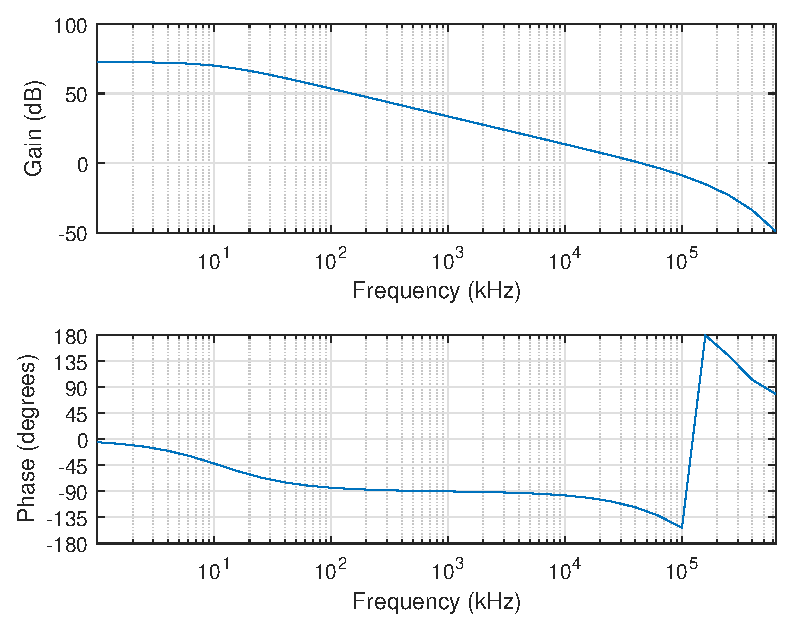
\includegraphics[width=0.8\columnwidth]{circuit/folded_cascode/ac_dm.eps}
  \caption{AC differential mode frequency response of the folded cascode operational amplifier.}
  \label{fig:folded_cascode_ac_dm}
\end{figure}

\begin{figure}[!htb]
  \centering
  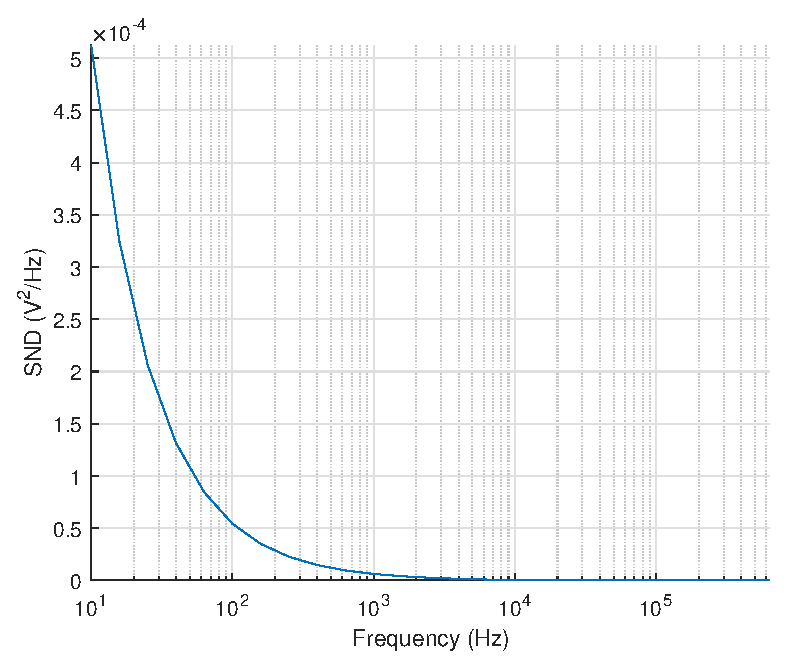
\includegraphics[width=0.8\columnwidth]{circuit/folded_cascode/ac_noise.eps}
  \caption{Output-referred AC noise of the folded cascode operational amplifier.}
  \label{fig:folded_cascode_ac_noise}
\end{figure}

\subsection{Comparator}

We then modified the operational amplifier to produce a comparator by removing $C_c$ and $R_c$ from \Cref{fig:folded_cascode}. The layout of this comparator is shown in \Cref{fig:comparator_layout}.

\begin{figure}[!htb]
  \centering
  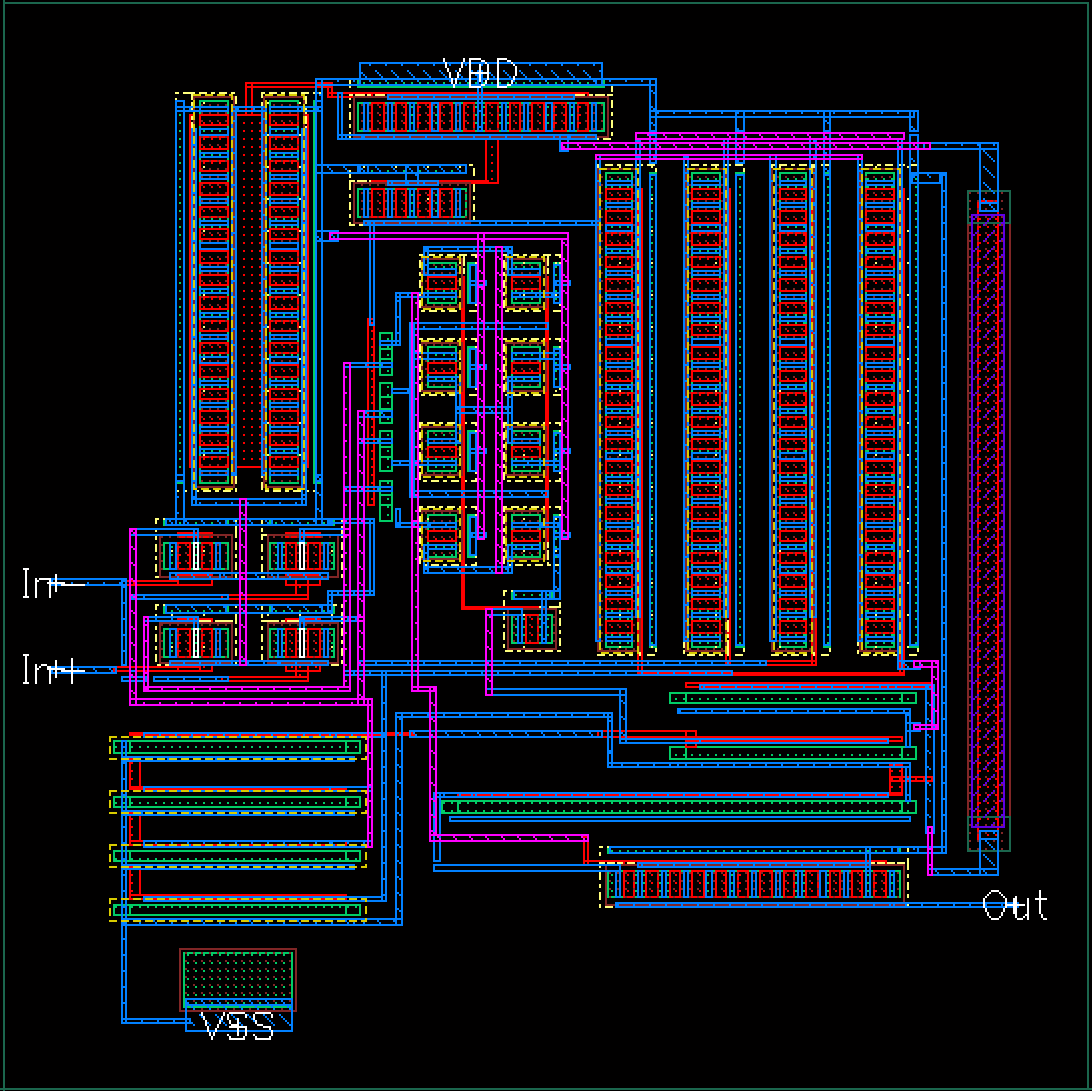
\includegraphics[width=0.8\columnwidth]{layout/comparator.png}
  \caption{A screenshot of the layout for the comparator.}
  \label{fig:comparator_layout}
\end{figure}

In the interest of creating a better Simulink model, we measured several parameters of the comparator. We found an offset voltage of $V_{os} = \SI{55}{\micro\volt}$, a DC gain of $A = \SI{4.28}{\kilo\volt\per\volt}$, and a bandwidth of $f_{3dB} = \SI{500.5}{\kilo\hertz}$. In addition, the open loop AC response and the output referred AC noise are shown in \Cref{fig:comparator_ac_dm,fig:comparator_ac_noise} respectively.

\begin{figure}[!htb]
  \centering
  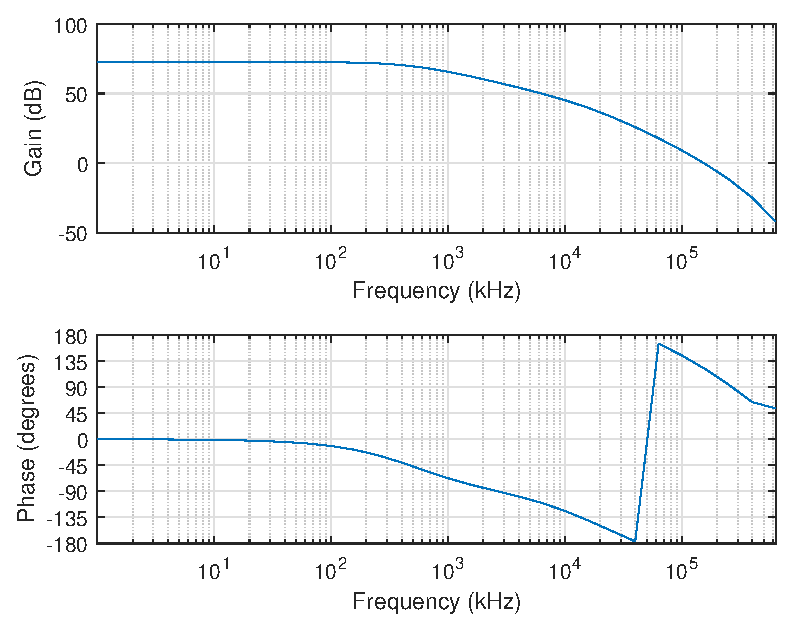
\includegraphics[width=0.8\columnwidth]{circuit/comparator/ac_dm.eps}
  \caption{AC differential mode frequency response of the comparator.}
  \label{fig:comparator_ac_dm}
\end{figure}

\begin{figure}[!htb]
  \centering
  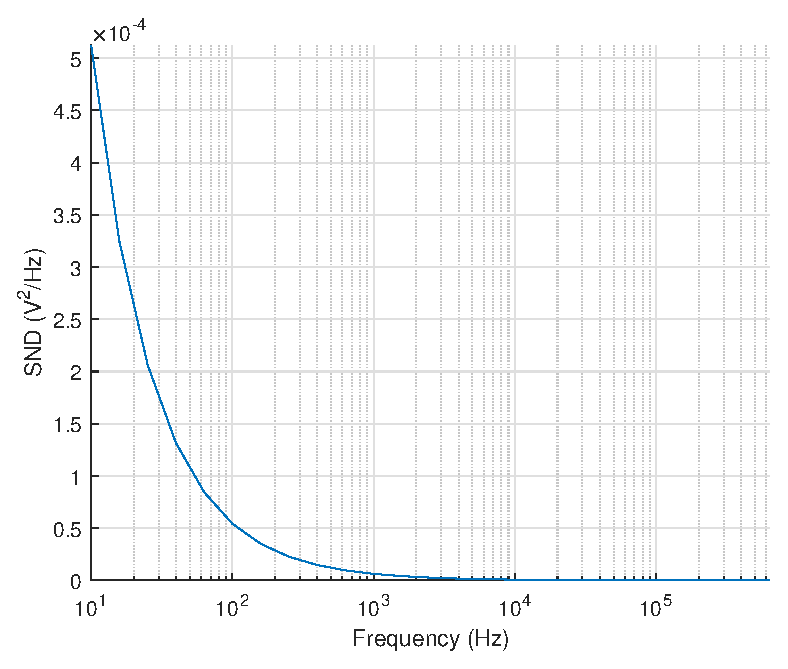
\includegraphics[width=0.8\columnwidth]{circuit/comparator/ac_noise.eps}
  \caption{Output-referred AC noise of the comparator.}
  \label{fig:comparator_ac_noise}
\end{figure}

\subsection{ADC}

With these subcomponents in hand, we then implemented the complete ADC, as shown in \Cref{fig:adc}. We chose values of $C_1 = C_2 = \SI{1.0}{\pico\farad}$ as a starting point. In addition, we used the reference voltages of $V_{ref+} = \SI{0.84}{\volt}$ and $V_{ref-} = \SI{0.36}{\volt}$ that were previously selected in the system level simulation. Note that instead of using $\Phi_1$ as the clock for the flip-flop, we used an inverted input clock. We did this to ensure that the clocks $\Phi_1$ and $\Phi_2$ drive equal loads so that they are equally delayed and do not overlap. An inverter was required to ensure that the flip-flop clock matches $\Phi_1$.

\begin{figure*}[!htb]
  \centering
  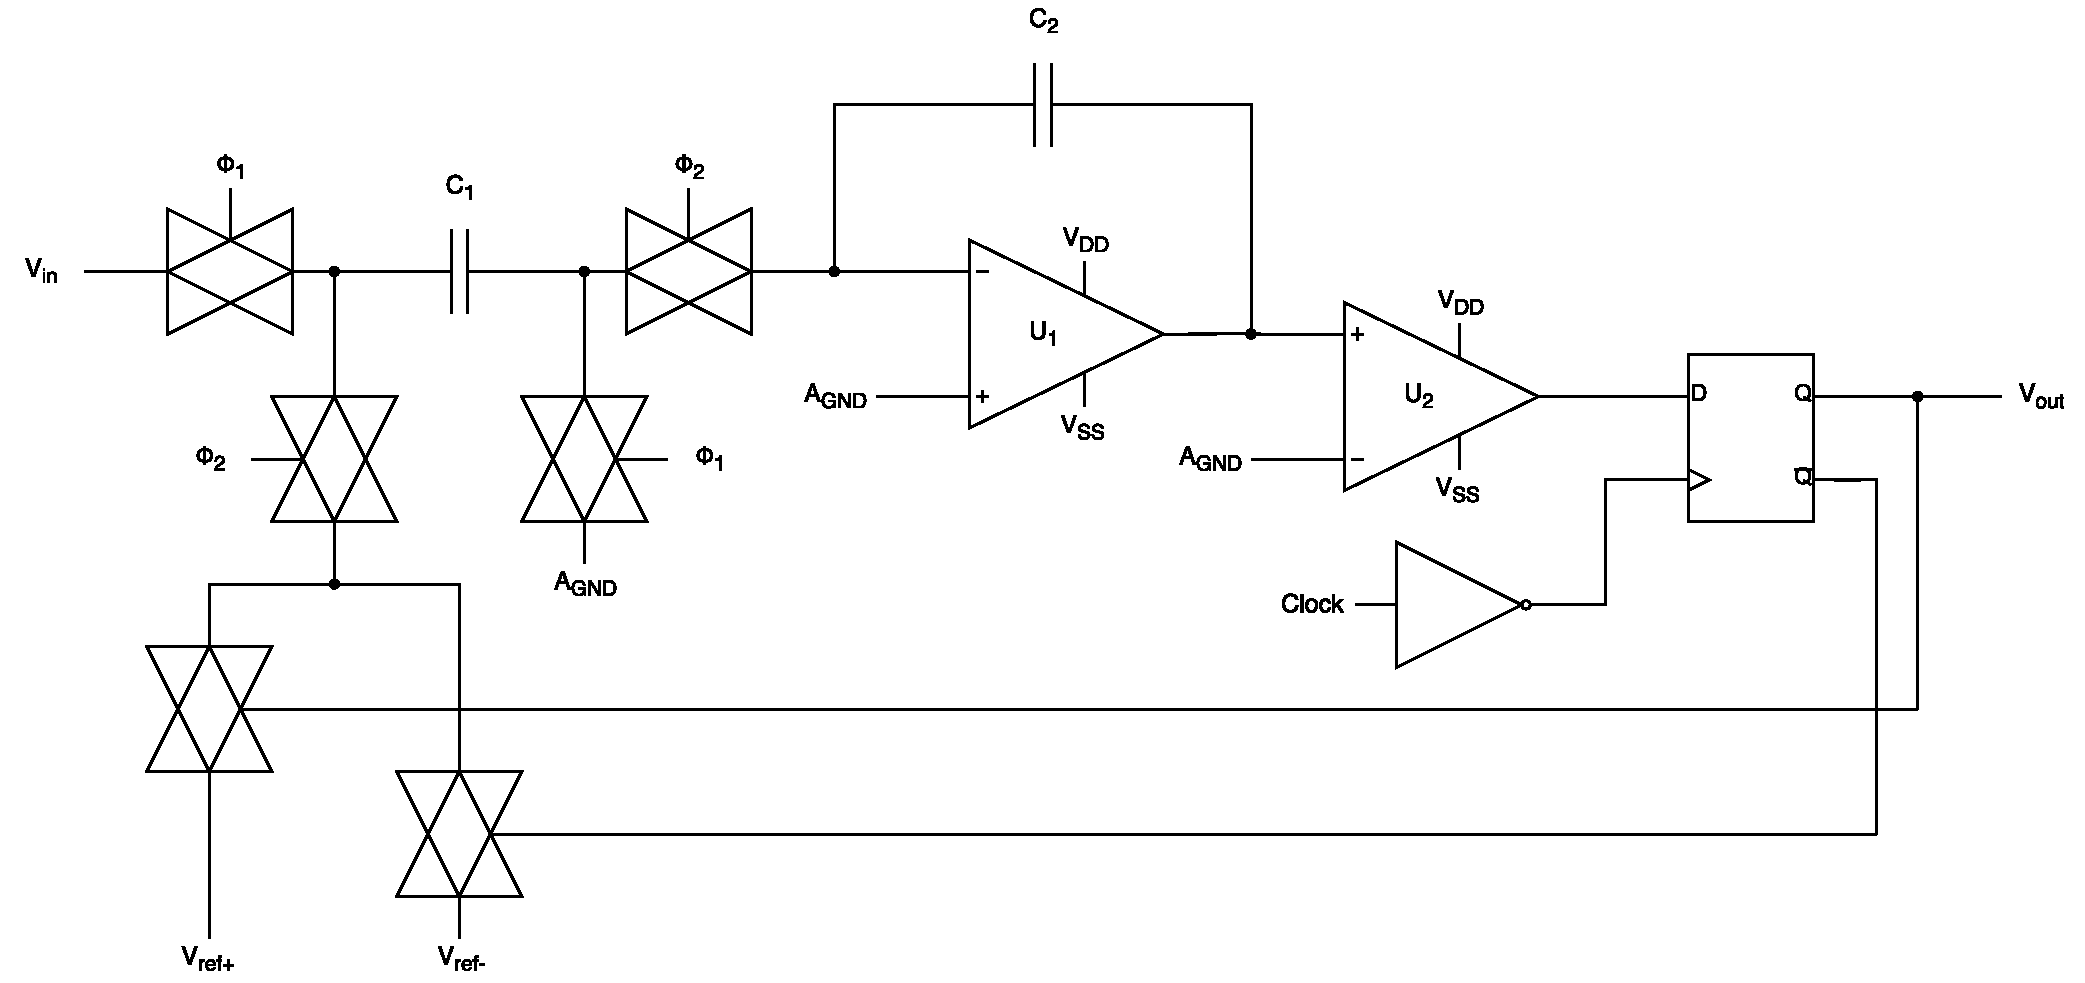
\includegraphics[width=\textwidth]{diagrams/adc.pdf}
  \caption{A schematic of the $\Delta \Sigma$ A/D converter.}
  \label{fig:adc}
\end{figure*}

We next performed a transient analysis of the circuit. As we did in our system level simulation, we used a $\SI{10}{\mega\hertz}$ clock and a $\SI{0.2}{\volt}$ amplitude, $\SI{20}{\kilo\hertz}$ sine wave input signal. We then ran the simulation for $\SI{2.1}{\milli\second}$ and discarded the first $\SI{0.1}{\milli\second}$, which allowed us to get $\SI{500}{\hertz}$ bins in our FFT. One issue we encountered was that the FFT expects uniform sampling while Cadence produces non-uniformly sampled outputs. To fix this, we set the \verb|strobeperiod| option of the transient simulation to $\SI{10}{\nano\second}$, which produces a uniformly sampled output and gives us 10 points per period of the sampling clock. In the FFT calculations, we then downsampled this output at our sampling frequency of $\SI{10}{\mega\hertz}$.

A plot of the power spectral density we obtained is shown in \Cref{fig:schematic_psd}. This figure shows that we obtained a SNDR of $\SI{65.4429}{\deci\bel}$ over our bandwidth of $\SI{38.22}{\kilo\hertz}$.

\begin{figure}[!htb]
  \centering
  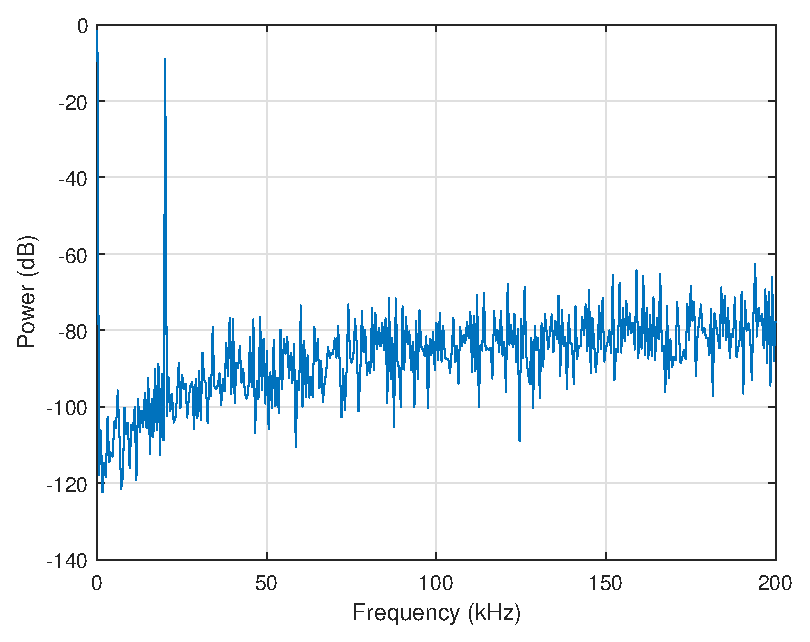
\includegraphics[width=0.8\columnwidth]{circuit/schematic_psd.eps}
  \caption{Power spectral density for the output of the schematic level simulation of the $\Delta \Sigma$ A/D converter.}
  \label{fig:schematic_psd}
\end{figure}

With the schematic level simulation meeting the specifications, we next moved on to layout. A screenshot of the complete layout is shown in \Cref{fig:adc_layout}, which measures $\SI{150}{\micro\meter}$ by $\SI{140}{\micro\meter}$ in total. We used several approaches to ensure good performance. First, the analog and digital parts were separated into their own sections of the IC. This ensures that the parasitic capacitance between these two parts of the circuit is low and thus that the large, fast digital signals do not couple with the small analog signals. In addition, the power supply lines were split between the two sections. A closer view of the digital section is shown in \Cref{fig:adc_digital_layout}.

\begin{figure}[!htb]
  \centering
  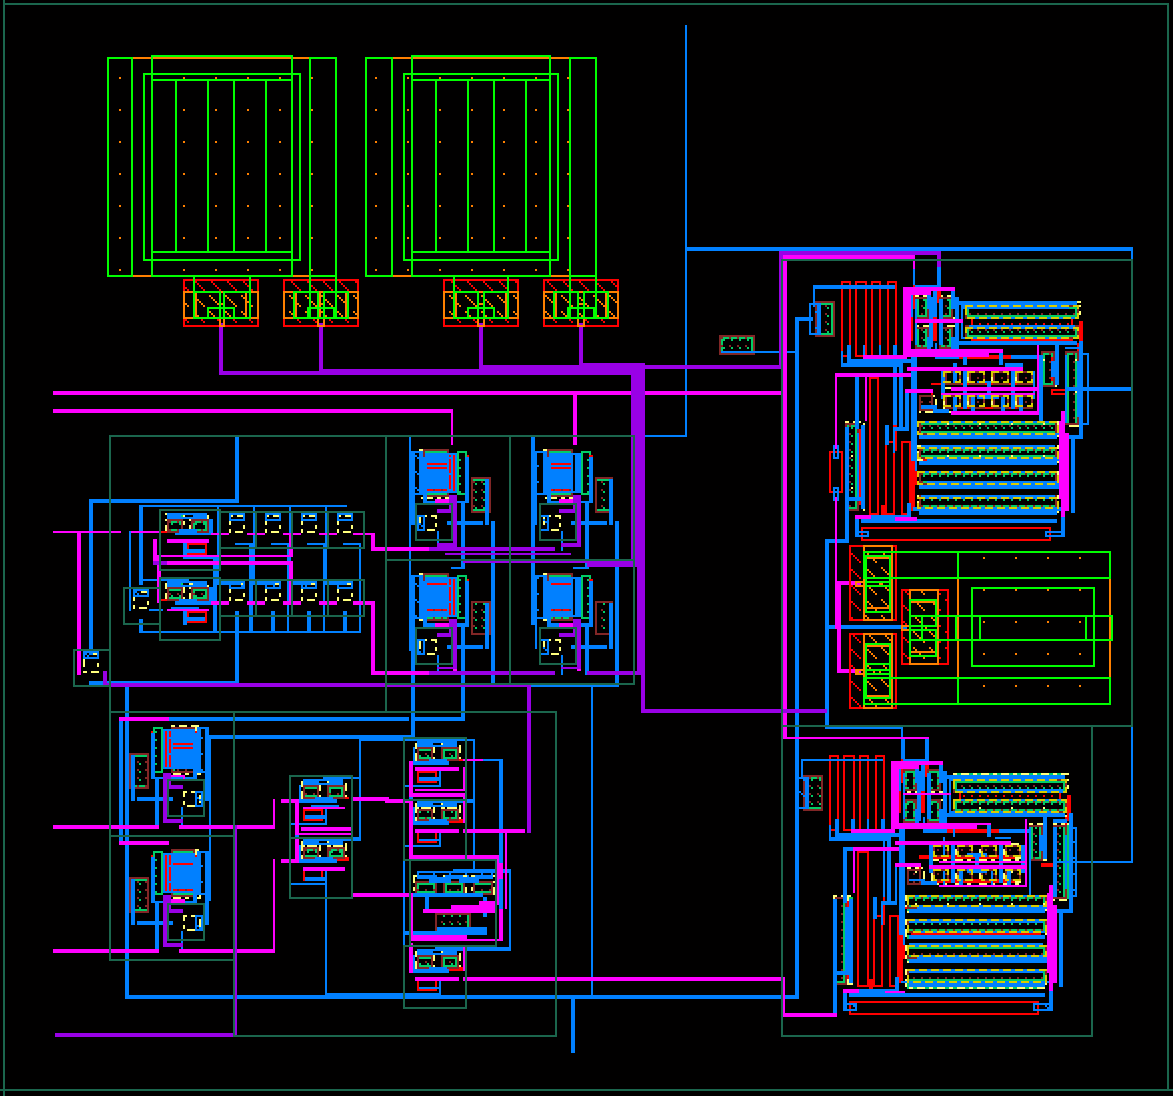
\includegraphics[width=\columnwidth]{layout/adc.png}
  \caption{A screenshot of the complete layout for the $\Delta \Sigma$ A/D converter.}
  \label{fig:adc_layout}
\end{figure}

\begin{figure}[!htb]
  \centering
  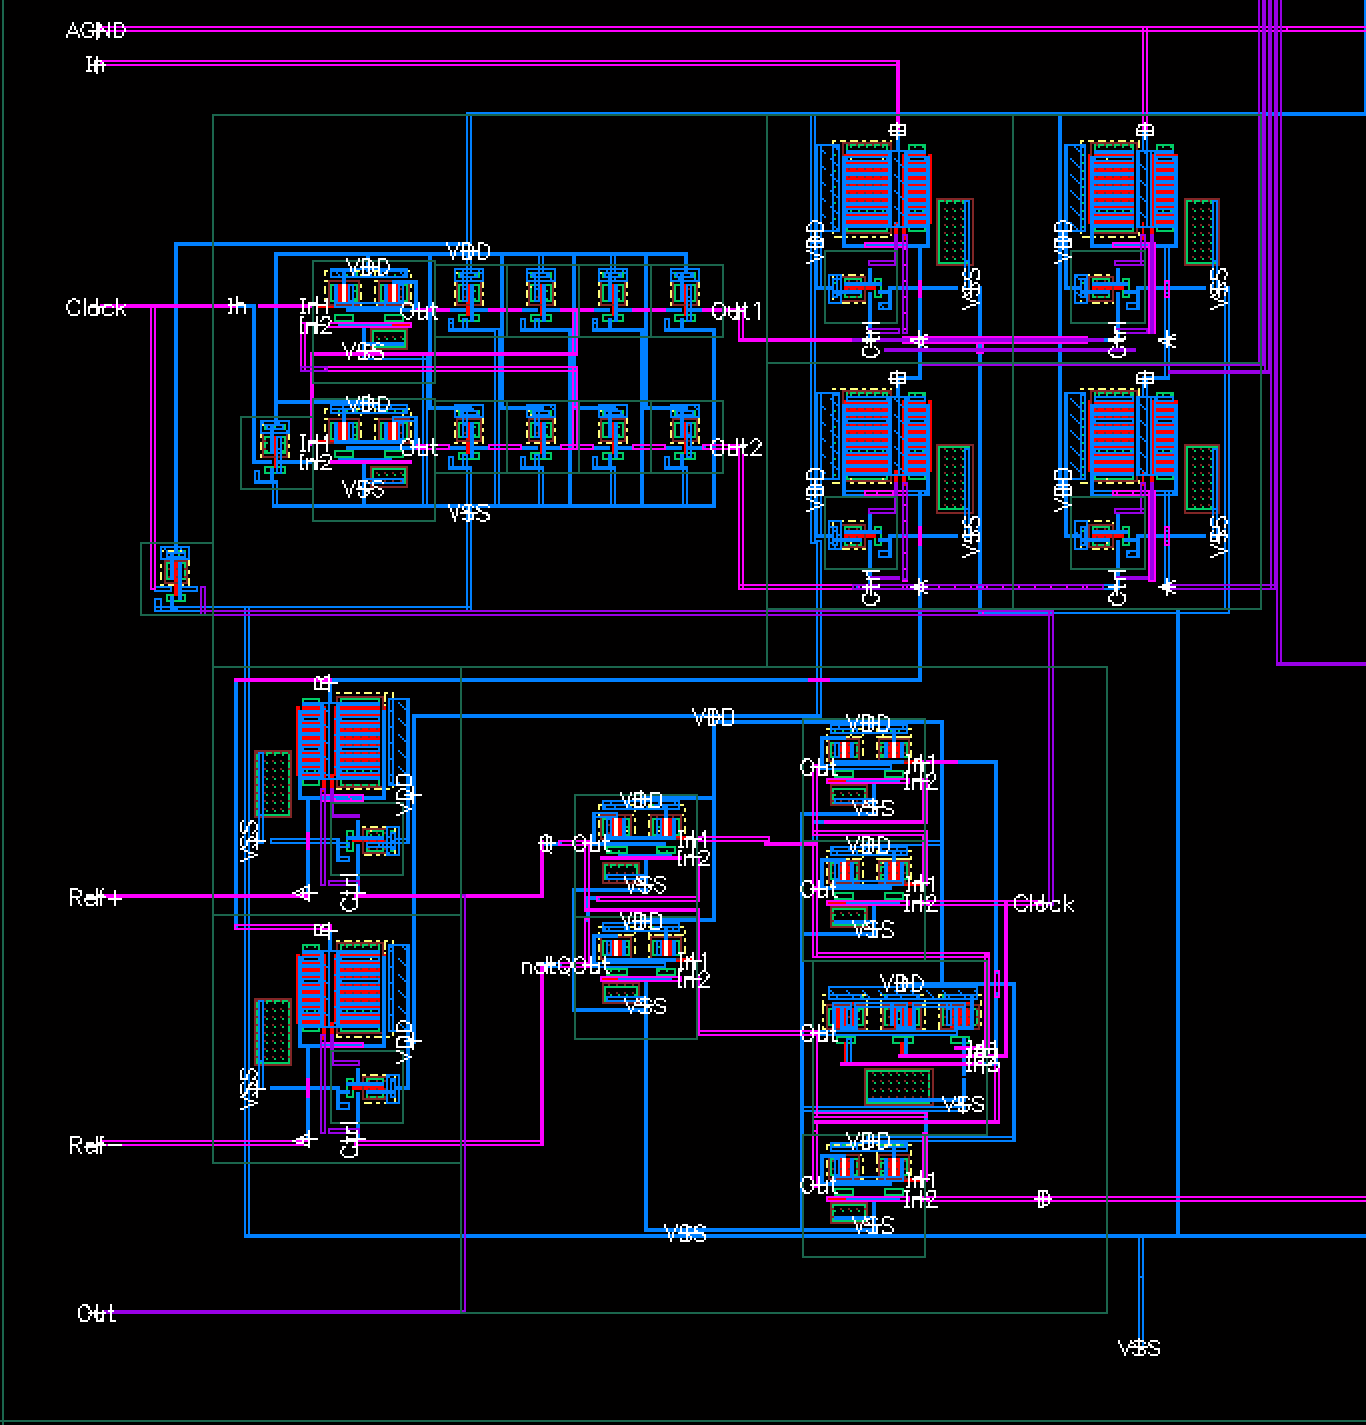
\includegraphics[width=\columnwidth]{layout/adc_digital.png}
  \caption{A screenshot of the layout of the digital components in the $\Delta \Sigma$ A/D converter.}
  \label{fig:adc_digital_layout}
\end{figure}

The other critical consideration was the intersection of analog and digital signals  that occurs in the transmission gates. In order to ensure that the small analog signals are not coupled to the large digital signals, we used shielding wherever these two types of signals got too close. An example is shown in \Cref{fig:adc_shielding_layout}, where $V_{SS}$ was extended to act as a shield between the clock signal $\Phi_1$ on the Ctrl line and the analog signal that passes from A to B.

\begin{figure}[!htb]
  \centering
  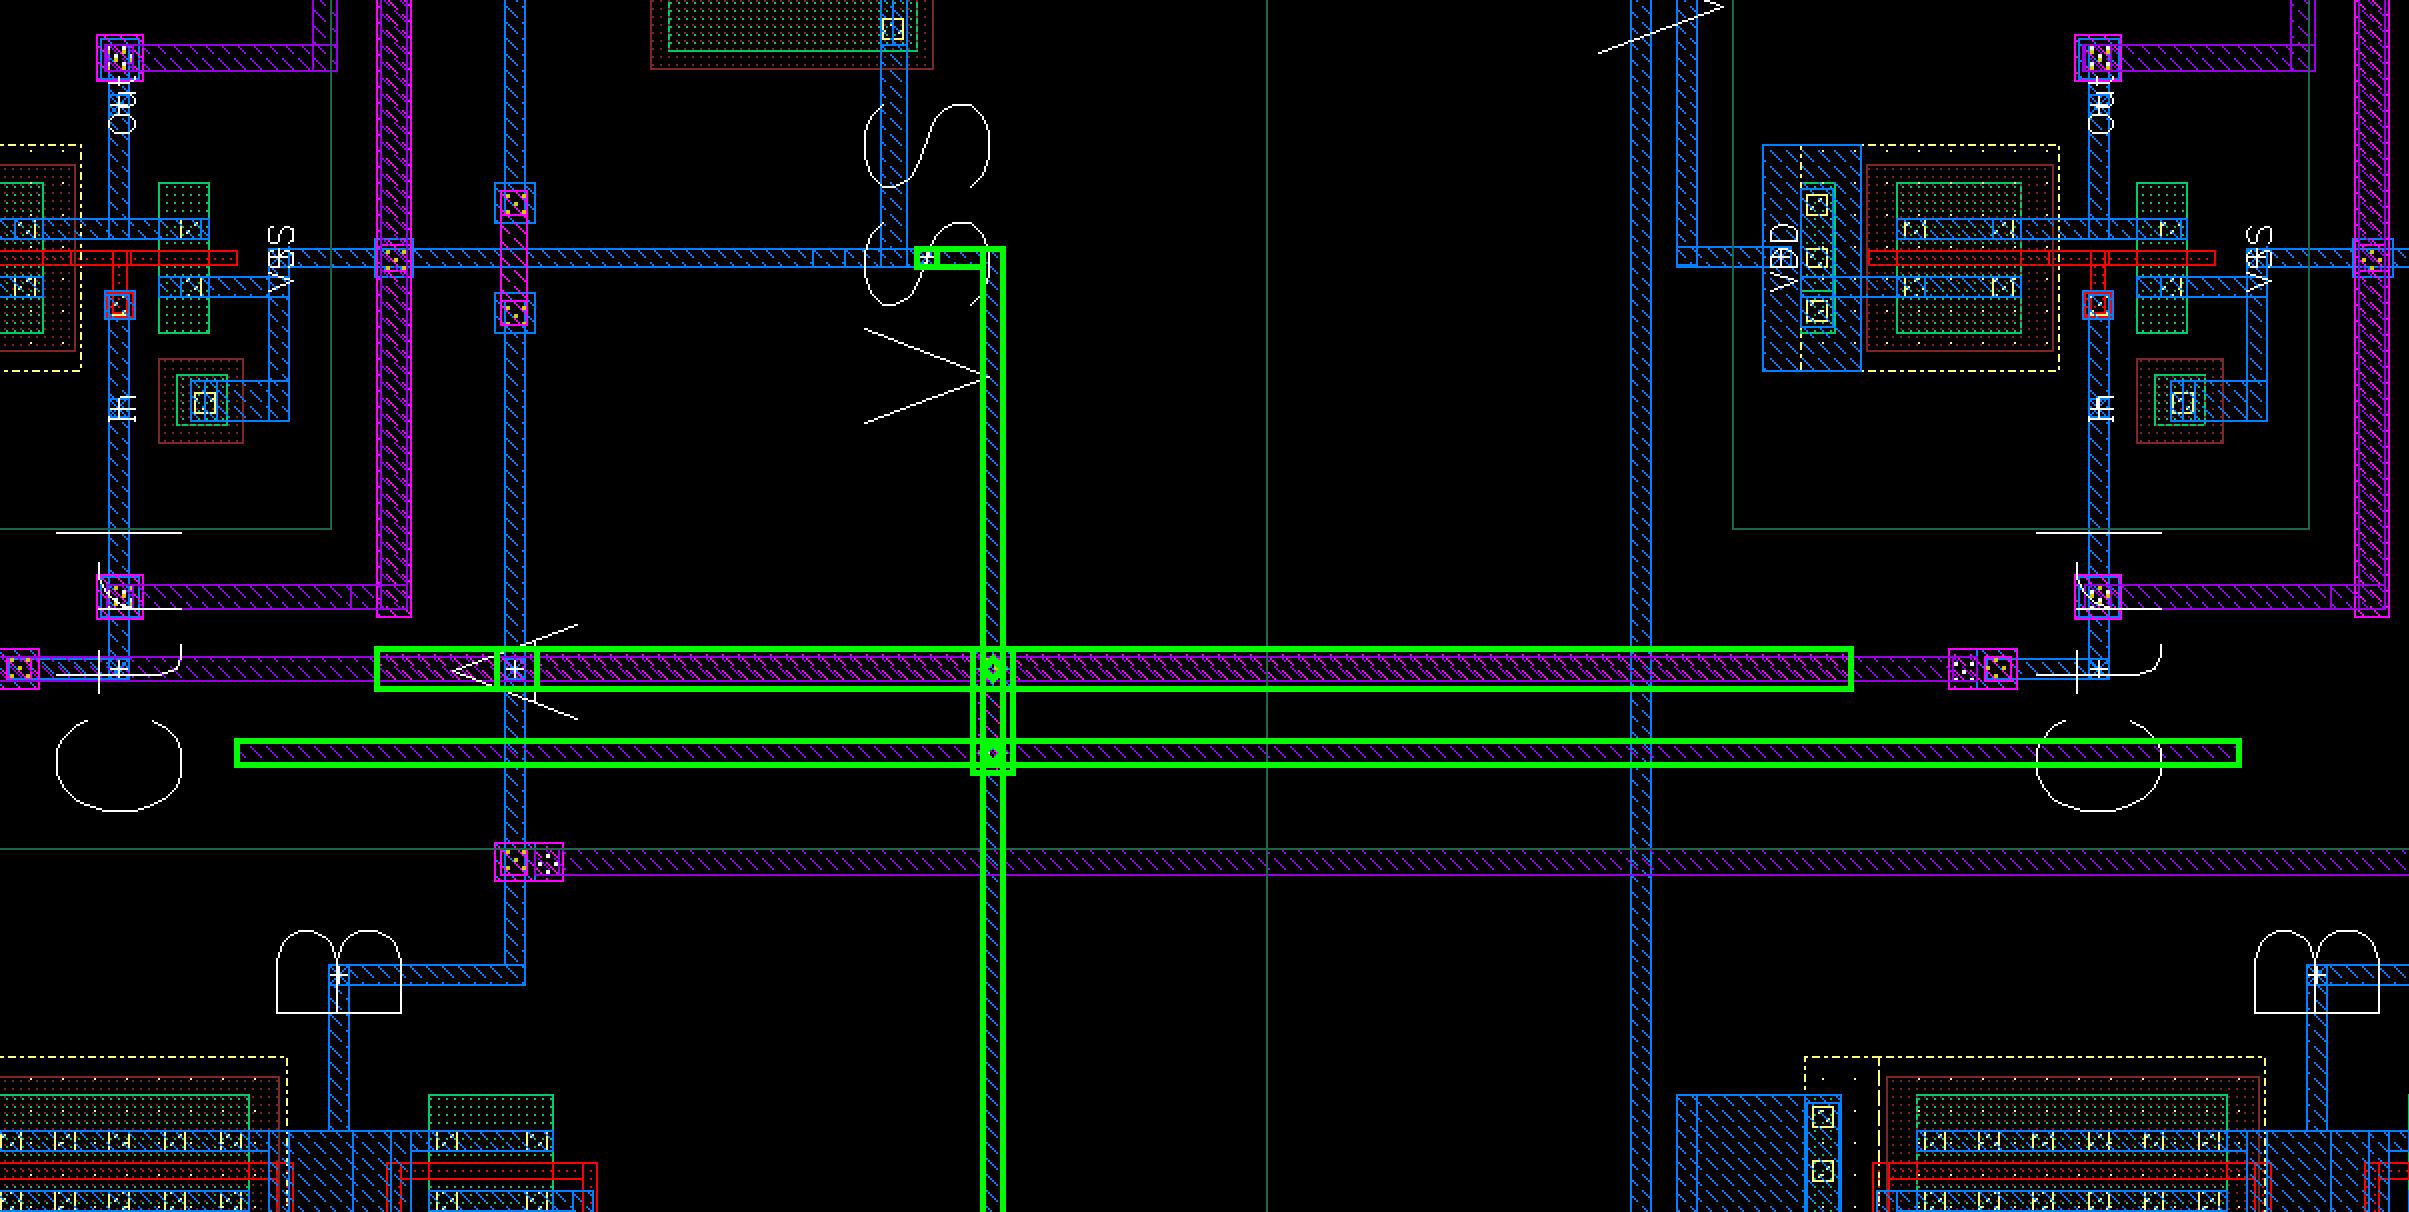
\includegraphics[width=0.8\columnwidth]{layout/adc_shielding.png}
  \caption{A screenshot of signal shielding in the layout of the $\Delta \Sigma$ A/D converter.}
  \label{fig:adc_shielding_layout}
\end{figure}

We then extracted the parasitics from this layout and performed a transient analysis of the circuit with the same parameters as for the schematic level simulation. A plot of the power spectral density we obtained is shown in \Cref{fig:layout_psd}. This figure shows that we obtained a SNDR of $\SI{60.3449}{\deci\bel}$ over our bandwidth of $\SI{38.22}{\kilo\hertz}$, which meets the specifications.

\begin{figure}[!htb]
  \centering
  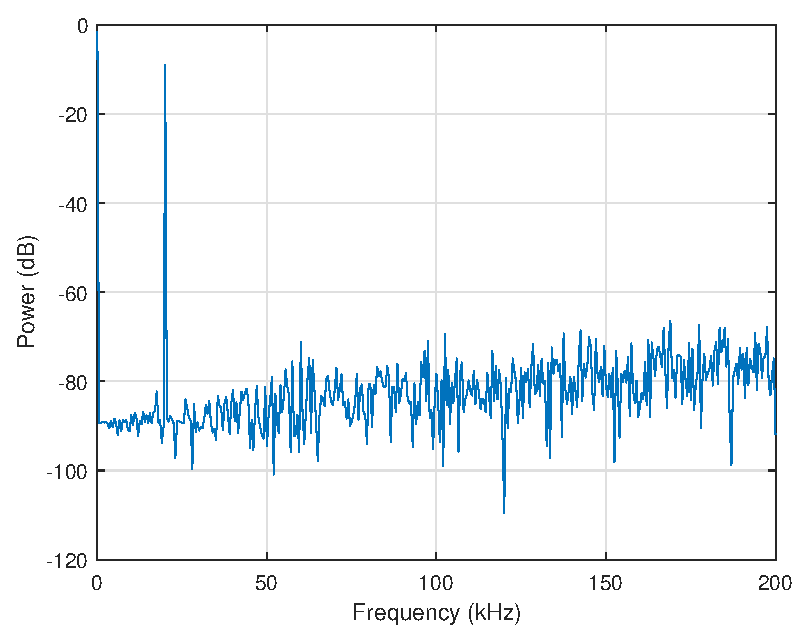
\includegraphics[width=0.8\columnwidth]{circuit/layout_psd.eps}
  \caption{Power spectral density for the output of the layout level simulation of the $\Delta \Sigma$ A/D converter.}
  \label{fig:layout_psd}
\end{figure}

A comparison of the PSD obtained for the different simulations is shown in \Cref{fig:comparison_psd}. This figure shows that the results obtained were similar across all simulations types, with the main difference occurring at the low frequencies. At these frequencies, the layout parasitics seem to have caused an increase in noise compared to the other two simulations. This translates to the decrease in SNDR from $\SI{63.7303}{\deci\bel}$ for the system level simulation and $\SI{65.4429}{\deci\bel}$ for the schematic level simulation to $\SI{60.3449}{\deci\bel}$ for the layout level simulation.

\begin{figure}[!htb]
  \centering
  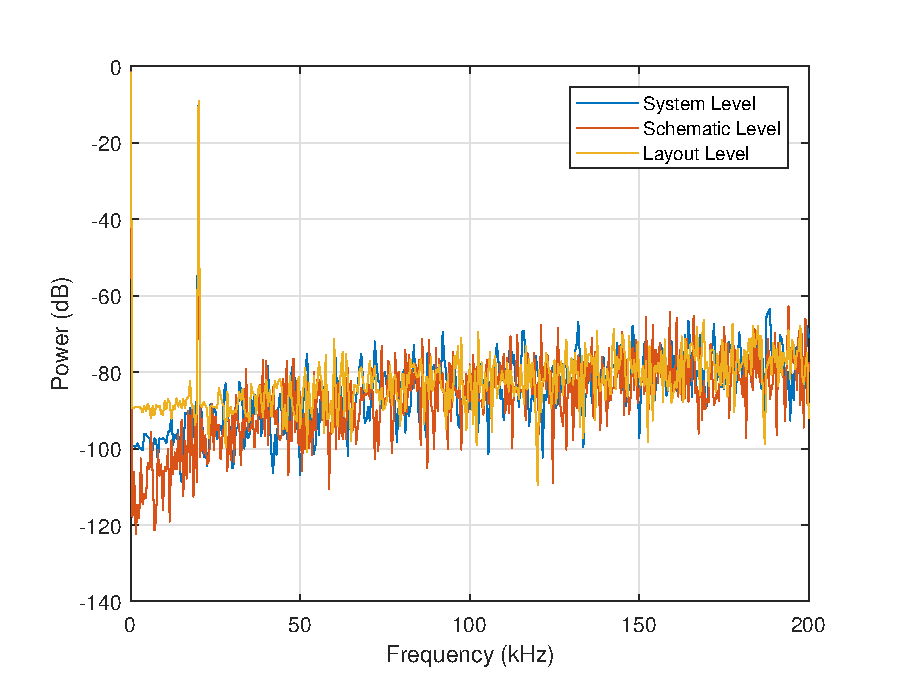
\includegraphics[width=0.8\columnwidth]{circuit/comparison_psd.eps}
  \caption{Power spectral density for the output of the $\Delta \Sigma$ A/D converter for different simulation types.}
  \label{fig:comparison_psd}
\end{figure}

To further characterize the performance of the ADC, we also measured the gain error and offset. We used MATLAB to create a FIR low pass digital filter with a pass-band frequency of $\SI{38.22}{\kilo\hertz}$, a stop-band frequency of $\SI{41.78}{\kilo\hertz}$, a pass-band ripple of $\SI{0.1}{\deci\bel}$, and a stop-band attenuation of $\SI{80}{\deci\bel}$. We then passed our output signal through this filter and measured the error when compared to the original signal.

The filtered output signal on a restricted time interval is shown in \Cref{fig:filtered_output}. The corresponding transfer characteristic is shown in \Cref{fig:gain_error_and_offset}. These figures show that the ADC produces a net offset of about $\SI{-4.38}{\milli\volt}$. In addition, the best fit curve through the transfer characteristic shows a gain of $1.0023$, which corresponds to a gain error of $\SI{0.23}{\percent}$.

\begin{figure}[!htb]
  \centering
  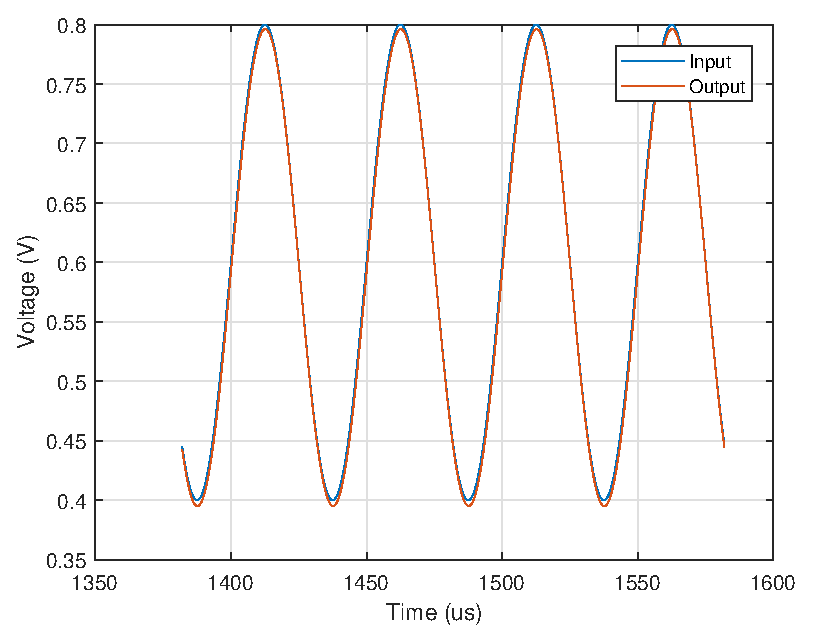
\includegraphics[width=0.8\columnwidth]{circuit/filtered_output.eps}
  \caption{Filtered output and input for the $\Delta \Sigma$ A/D converter.}
  \label{fig:filtered_output}
\end{figure}

\begin{figure}[!htb]
  \centering
  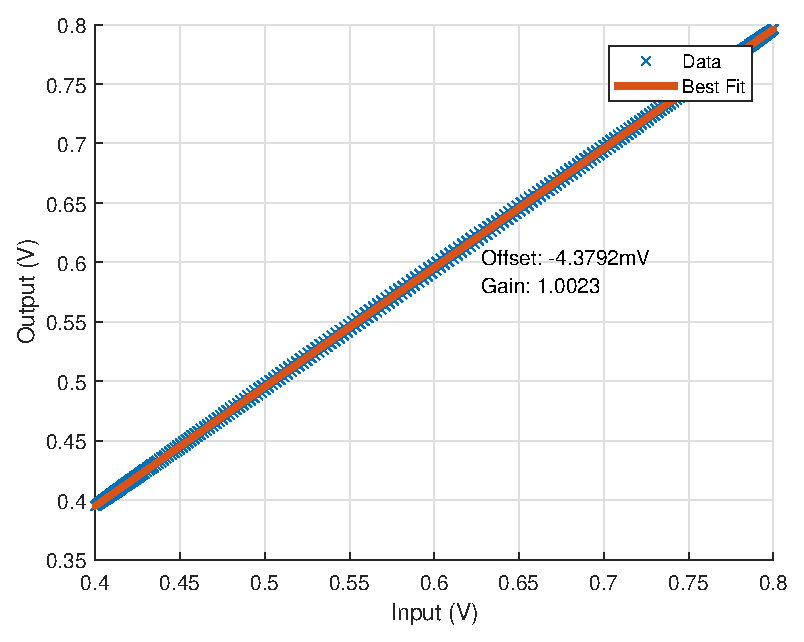
\includegraphics[width=0.8\columnwidth]{circuit/gain_error_and_offset.eps}
  \caption{Filtered output vs. input for the $\Delta \Sigma$ A/D converter.}
  \label{fig:gain_error_and_offset}
\end{figure}

We next plotted the error with offset subtracted against the input signal value, as shown in \Cref{fig:error}. This figure shows that the error has a circular shape, which suggests that it is not actually an error but a phase delay in the signal. In fact, we can compute the value of the delay as $A sin(\phi) = \epsilon$, where $A$ is the input signal amplitude and $\epsilon$ is the error with no input. The result is that $\phi = \SI{1.06}{\degree}$, so the total time delay is $\tau = \SI{147}{\nano\second}$, which matches the delay observed in \Cref{fig:filtered_output}.

\begin{figure}[!htb]
  \centering
  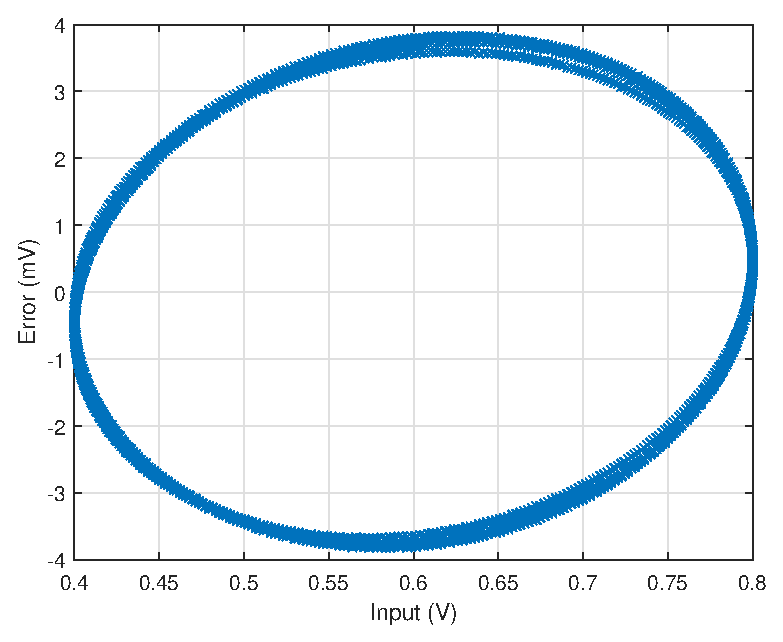
\includegraphics[width=0.8\columnwidth]{circuit/error.eps}
  \caption{Error with offset subtracted vs. input for the $\Delta \Sigma$ A/D converter.}
  \label{fig:error}
\end{figure}

Finally, we measured the power supply current over a $\SI{50}{\micro\second}$ time period and multiplied it by $V_{DD} = \SI{1.2}{\volt}$ in order to calculate the circuit's power dissipation. Partial results are shown in \Cref{fig:layout_power}. We can see that large spikes occur when the circuit's digital components are switching. The peak power dissipation is therefore $\SI{837}{\micro\watt}$. Integrating the curve and dividing by the interval yields an average power dissipation of $\SI{194}{\micro\watt}$.

\begin{figure}[!htb]
  \centering
  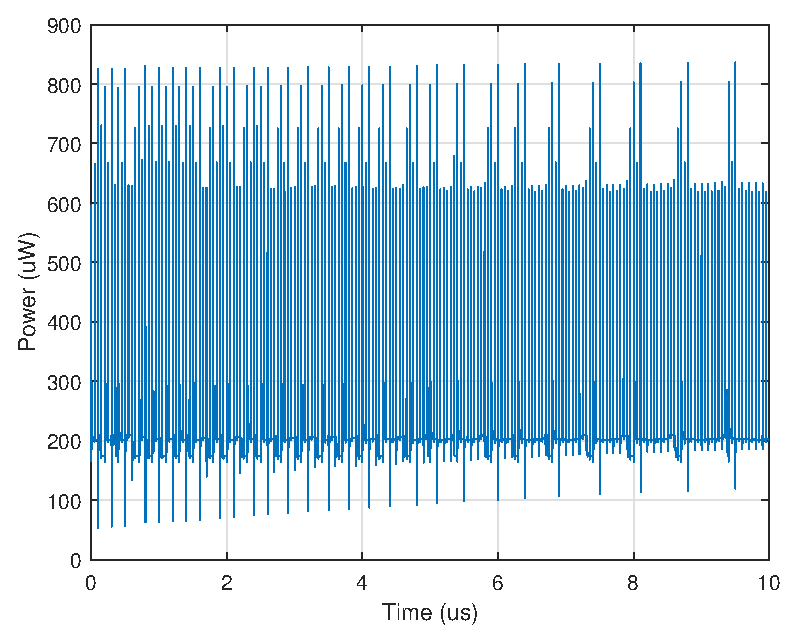
\includegraphics[width=0.8\columnwidth]{circuit/layout_power.eps}
  \caption{Power dissipation of the $\Delta \Sigma$ A/D converter.}
  \label{fig:layout_power}
\end{figure}

Since we were not given a quantitative requirement for power dissipation, we can evaluate our implementation by comparing our average power dissipation of $\SI{194}{\micro\watt}$ to the Assignment \#2 maximum of $\SI{200}{\micro\watt}$ for a single operational amplifier. This comparison shows that our power dissipation is quite low, given that our combined circuit consumes less power on average than the maximum we were given for a single operational amplifier.

\section{Conclusions}

In conclusion, we designed, simulated, laid out, and analyzed a first order, single bit, $\Delta \Sigma$ A/D converter using MATLAB and Cadence. To meet our specifications of a $\SI{38.22}{\kilo\hertz}$ bandwidth and a peak SNDR of at least $\SI{60}{\deci\bel}$, we used a sampling frequency of $\SI{10}{\mega\hertz}$. We then chose DAC output voltage levels of $\SI{0.36}{\volt}/\SI{0.84}{\volt}$ in order to maximize the SNDR while taking PVT into account. With these parameters, our system level simulation yielded a SNDR of $\SI{63.7303}{\deci\bel}$, our schematic level simulation yielded a SNDR of $\SI{65.4429}{\deci\bel}$, and our layout level simulation yielded a SNDR of $\SI{60.3449}{\deci\bel}$. Therefore, our A/D converter satisfies all the given requirements.

\bibliographystyle{IEEEtran}
\bibliography{IEEEabrv,references}

\end{document}
